% =========================
% Overleaf (IEEE) Template
% Paper 2: WAAM Geometry Mapping
% =========================
% Upload this as main.tex in Overleaf and compile with PDFLaTeX.
% If you want BibTeX references, also upload refs.bib (provided below).

\documentclass[conference]{IEEEtran}

% =========================
% PACKAGES
% =========================
\usepackage[utf8]{inputenc}     % Allow UTF-8 characters
\usepackage[T1]{fontenc}        % Font encoding for better characters
\usepackage{lmodern}            % Modern font family
\usepackage{amsmath, amssymb, amsfonts}  % For mathematical symbols and fonts
\usepackage{graphicx}           % For including images
\usepackage{booktabs}           % For better tables
\usepackage{multirow}           % For multi-row tables
\usepackage{siunitx}            % For SI units formatting
\usepackage{url}                % For URLs
\usepackage[numbers,sort&compress]{natbib} % For citations
\usepackage{newunicodechar}
\newunicodechar{\nobreakspace}{~} % Handle U+202F NARROW NO-BREAK SPACE

% Optional Packages
\usepackage{float}              % For better floating elements (tables/figures)
\usepackage{hyperref}           % For hyperlinks and cross-referencing

% =========================
% DOCUMENT START
% =========================

\begin{document}
% -------------------------
% Title / Authors
% -------------------------
\title{Multivariable Influence of Process Parameters on Bead Geometry in Wire Arc Additive Manufacturing}

\author{
\IEEEauthorblockN{
Bathlomew Ebika$^{1}$,
Vishnu Ramasamy$^{1,3}$,
John Lewandowski$^{2}$,
Kenneth A. Loparo$^{1}$
Jacob Ekeamadi$^{4}$
}

\IEEEauthorblockA{
$^{1}$Department of Electrical, Computer and Systems Engineering, Case Western Reserve University, Cleveland, OH, USA
}

\IEEEauthorblockA{
$^{2}$Department of Materials Science and Engineering, Case Western Reserve University, Cleveland, OH, USA
}

\IEEEauthorblockA{
$^{3}$Department of Materials Science \& Engineering, Ohio State University, Columbus, OH, USA
}
\IEEEauthorblockA{
$^{4}$Peatech Institute for Intelligent Systems, Cleveland, OH, USA
}

\IEEEauthorblockA{
\texttt{bae54@case.edu, kal4@case.edu, jjl3@case.edu, vxv191@case.edu, jacob@peatechservice.com}
}
}

\maketitle


% -------------------------
% Abstract / Keywords
% -------------------------
\begin{abstract}

Wire Arc Additive Manufacturing (WAAM) relies on the coordinated control of electrical and kinematic parameters to achieve consistent bead geometry and stable deposition. However, the combined influence of voltage (V), wire feed speed (WFS), travel speed (TS), and contact tip‑to‑work distance (CTWD) remains insufficiently characterized across materials and operating ranges. This study presents an experimental analysis based on 796 single‑bead depositions, performed on two materials (AISI 316 stainless steel and ER70S‑6 low‑carbon steel), where four process parameters were systematically varied and bead height, bead width, and variance‑based stability metrics were extracted from high‑resolution profilometry.

The results show that changes in heat input—arising from combinations of V, WFS, TS, and CTWD—produce material‑dependent geometric responses, with stainless steel exhibiting greater spreading at high heat input and low carbon steel showing more confined bead formation due to faster thermal dissipation. Variance‑based metrics reveal distinct ranges of stable, marginal, and unstable deposition behavior, defined empirically by increases in height and width variance rather than by assumed nonlinear interactions. CTWD is shown to influence interfacial bonding through its effect on current and heat input, enabling either strong adhesion or reduced bonding suitable for controlled first‑layer detachability.

Overall, the study provides an experimentally grounded process–geometry mapping that links measurable heat‑input changes to geometric and stability outcomes across materials. These findings offer a practical basis for parameter selection and future development of predictive or closed‑loop WAAM control strategies.
\end{abstract}

\begin{IEEEkeywords}
Wire Arc Additive Manufacturing (WAAM), bead geometry, process parameters, variance-based metrics, interfacial bonding, contact tip-to-work distance (CTWD), material-dependent behavior, stainless steel, low-carbon steel.
\end{IEEEkeywords}

\section{Introduction}

Additive manufacturing has emerged as a transformative manufacturing paradigm, enabling the fabrication of complex geometries through layer-by-layer material deposition, while offering unprecedented flexibility, scalability, and process customization. \cite{salinas2023blockchain,Lewandowski2016Review}. 

Wire Arc Additive Manufacturing (WAAM) offers a high‑deposition pathway for producing large metal components, but its performance depends critically on how electrical and kinematic parameters shape bead geometry and deposition stability. However, comparatively fewer studies have evaluated these parameters within a common experimental framework across multiple materials while simultaneously examining mean bead geometry and along-bead geometric variability. This limits the development of reliable process–geometry relationships and constrains efforts toward predictive or closed‑loop WAAM control.

To address this gap, the present work conducts a broad experimental evaluation of how these parameters affect bead geometry and stability in WAAM. Using 796 single‑bead depositions across AISI316 stainless steel and ER70S‑6 low‑carbon steel, the study integrates geometric measurements with variance‑based stability metrics and interprets the results through the lens of heat‑input‑driven melt‑pool behavior.

This paper makes three primary contributions. They are;

(i). A multivariable experimental assessment of voltage (V), wire feed speed (WFS), travel speed (TS), and contact tip‑to‑work distance (CTWD) across two materials using a traceable registry of 796 single-bead deposition runs, including 480 runs with complete longitudinal height descriptors and a nested subset of 247 runs with paired multi-level width measurements.

(ii). Integration of mean bead geometry with variance‑based stability metrics, enabling a unified evaluation of geometric outcomes and deposition consistency.

(iii). A physics‑informed interpretation linking parameter changes to heat input and material‑dependent geometric response, establishing an evidence‑based process–geometry mapping for WAAM.

\section{The Evolution of WAAM Process Parameters: A Historical Perspective}

The development of Wire Arc Additive Manufacturing (WAAM) has progressed from basic arc-based metal deposition toward increasingly controlled, adaptive, and data-driven processes. Early work by Baker in 1920 demonstrated the feasibility of producing three-dimensional metallic structures through controlled deposition using an electrical arc and a fusible electrode, establishing the fundamental relationship between deposition rate, electrical input, and travel speed \cite{Baker1925}. Subsequent developments in the 1990s shifted attention toward systematic control of process parameters, including the relationship between Wire Feed Speed (WFS), Travel Speed (TS), and inter-pass conditions for improving dimensional stability \cite{Dickens1992}.

The introduction of feedback control represented a further transition from fixed process parameters toward adaptive deposition. Spencer et al. demonstrated the use of real-time monitoring and dynamic adjustment of deposition conditions to compensate for variations in deposited height \cite{Spencer1998}. Later developments expanded process control beyond electrical and kinematic parameters. Work at Cranfield University demonstrated the use of inter-pass rolling to modify the deposited material and improve structural performance through controlled mechanical deformation \cite{Williams2016}. More recently, predictive and machine-learning approaches have enabled process parameters such as travel speed and deposited layer height to be dynamically adjusted based on evolving process conditions \cite{Xiong2014}.

This progression reflects a broader transition in WAAM from empirical parameter selection toward integrated process monitoring, adaptive control, and predictive modeling. However, despite these advances, the coupled influence of multiple process parameters and the material-dependent nature of their effects remain important challenges. In particular, a systematic understanding of how voltage, WFS, TS, and contact tip-to-work distance (CTWD) jointly influence bead geometry and deposition stability is still required. This motivates the multivariable, material-aware analysis presented in this study.

\section{Research Gap and Motivation}

Despite significant advances in WAAM process monitoring, parameter optimization, and adaptive control, several challenges remain in establishing a comprehensive understanding of the relationship between process parameters, material behavior, and bead geometry \cite{Xiong2014,Guo2021MLAM,Sharma2022PhysicsML}. Many existing studies simplify the process space by examining limited parameter combinations or focusing on individual process variables, which can make it difficult to capture the coupled effects that govern deposition behavior \cite{mansor2024waam_opt,Lambiase2022,Karmuhilan2018}.

First, the interaction among key process parameters remains insufficiently characterized. Voltage ($V$), wire feed speed (WFS), travel speed (TS), and contact tip-to-work distance (CTWD) influence heat input, deposition rate, and melt pool behavior simultaneously. Changes in one parameter can therefore alter the effect of others, making single-parameter interpretations inadequate for describing the full process--geometry relationship \cite{mansor2024waam_opt,debroy2018,jain2026}. In this study, these parameters are examined within a common experimental framework to establish their combined influence on bead height, bead width, and geometric variability.

Second, bead geometry is commonly evaluated using average dimensional characteristics, while variations along the deposited bead receive comparatively less attention. Mean bead height and width alone may not adequately distinguish between geometrically consistent and unstable deposition conditions 
\cite{Lambiase2022,Karmuhilan2018,song2012control}. Process monitoring and control studies have demonstrated the importance of deposition-height consistency and process stability for reliable WAAM operation, particularly in multilayer deposition
\cite{Colegrove2013HighPressureRolling,Craeghs2011Monitoring}. To address this limitation, the present study incorporates variance-based geometric metrics to quantify fluctuations in bead height and width and provide an additional measure of deposition stability.

Third, the response of WAAM to identical process conditions can differ substantially between materials because of differences in thermal conductivity, thermal diffusivity, melting behavior, and melt pool dynamics \cite{debroy2018,Guo2021MLAM,Sharma2022PhysicsML}. Consequently, process-geometry relationships established for one material cannot necessarily be generalized to another. This study therefore compares AISI 316 stainless steel and ER70S-6 low-carbon steel under corresponding process conditions to identify material-dependent differences in bead formation and geometric stability
\cite{jain2026,Le2022,Lewandowski2016Review}.

Finally, CTWD represents an important process variable because changes in wire extension alter electrical resistance, welding current, and consequently the effective heat input delivered during deposition \cite{jain2026,ebika2020waam}. Its influence on bead geometry and first-layer interfacial behavior therefore warrants specific consideration. The present study evaluates CTWD alongside the other process parameters to examine its effect on heat input, bead geometry, and the resulting interfacial response \cite{ding2015,jain2026}.

Accordingly, this study addresses these gaps through a multivariable experimental investigation of voltage, WFS, TS, and CTWD for AISI 316 and ER70S-6. The analysis combines bead height and width with variance-based stability measures and a heat-input framework to establish a material-aware relationship between process conditions and geometric response. The resulting framework provides a basis for more systematic parameter selection and supports future development of predictive and closed-loop WAAM process control strategies \cite{Guo2021MLAM,Sharma2022PhysicsML}.



\begin{figure*}[!t]
    \centering
    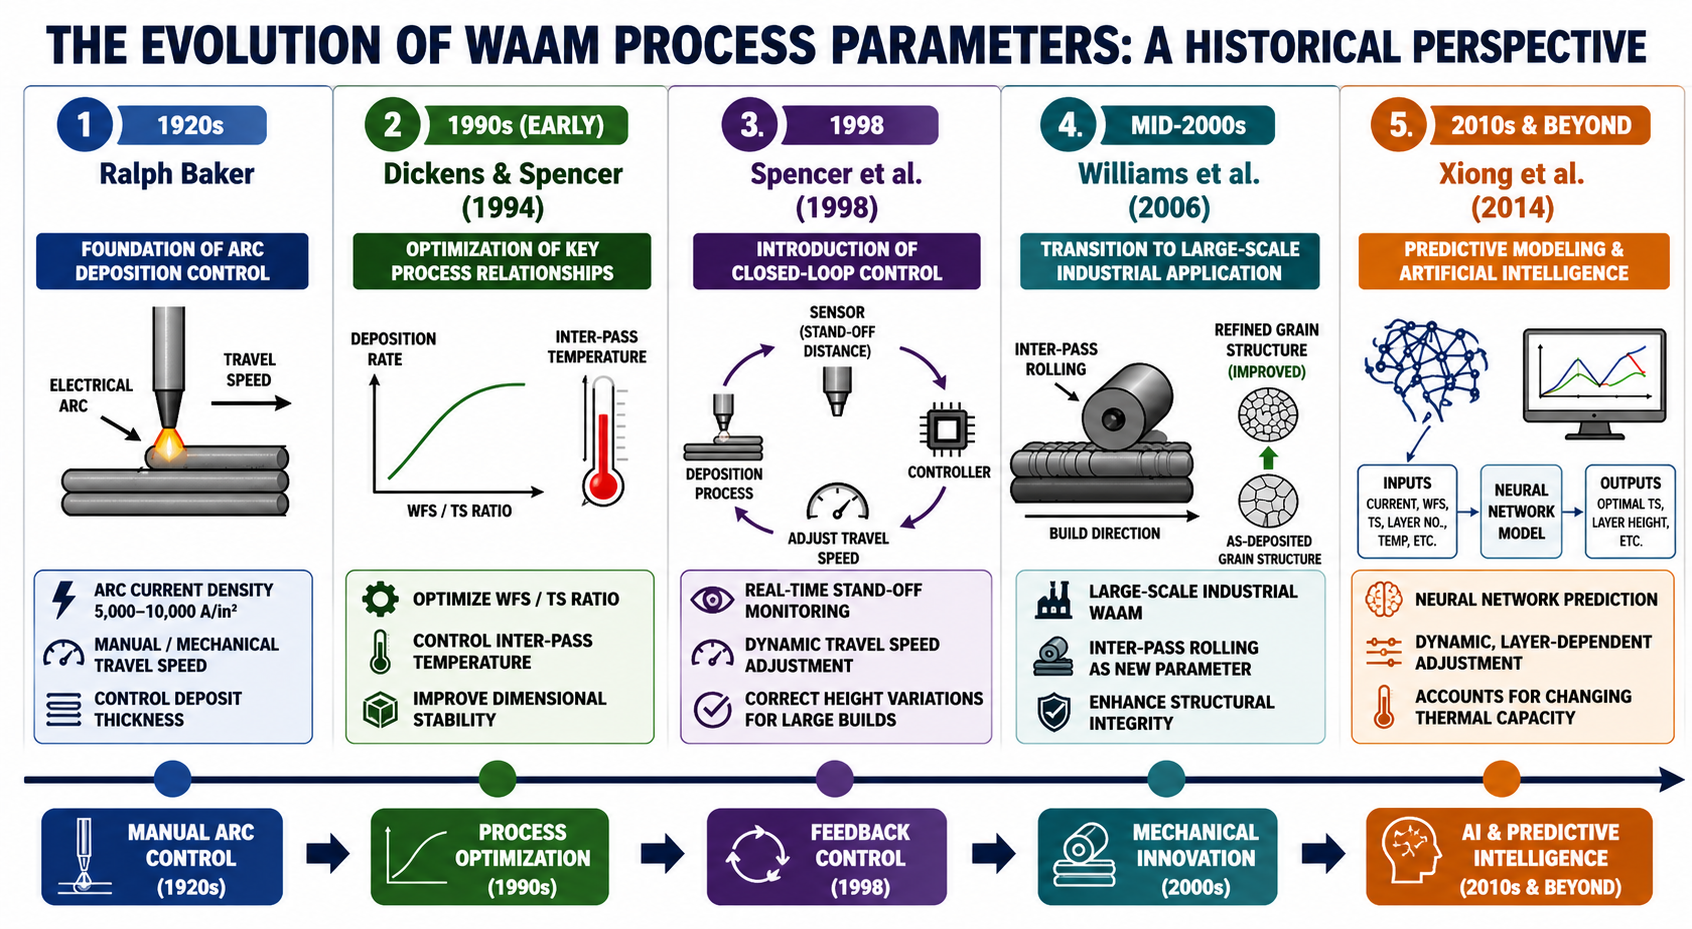
\includegraphics[width=4.00\textwidth,height=0.39\textheight,keepaspectratio]{qq.png}
    \caption{Evolution of WAAM Process Parameter}
    \label{fig:waam_setup}
\end{figure*}


\section{Multiphysics Basis for Interpreting Experimental Trends} 

Understanding how WAAM process parameters influence bead geometry traditionally involves a multiphysics description that couples electrical power input, heat transfer, molten‑pool fluid flow, Marangoni convection, and free‑surface evolution. These governing equations establish the physical mechanisms through which voltage, wire feed speed, travel speed, and CTWD affect melt‑pool size and bead morphology. In this study, these equations are presented only as a conceptual framework for interpreting the experimental results; they are not solved numerically, nor is a full multiphysics simulation implemented.

Instead, the analysis relies on a reduced‑order heat‑input relationship, expressed in Eq.20, which links measurable electrical parameters to the thermal energy delivered to the substrate. This formulation captures the dominant physics governing melt‑pool expansion, bead spreading, and material‑dependent geometric response. 
Grounding the interpretation in Eq.20 allows the study to translate parameter adjustments into predictable changes in bead height, width, and stability variance, providing a clear, physics‑based explanation for the trends observed across the available validated experimental observations. The multiphysics equations therefore serve as physical justification, while Eq.20 provides the operative model used to explain how voltage, WFS, TS, and CTWD collectively shape WAAM deposition behavior.

\subsection{Electrical Power and Arc Energy Transfer}

The instantaneous electrical power supplied to the arc is

\begin{equation}
P_{\mathrm{elec}}(t) = V(t) I(t)
\label{eq:elec_power}
\end{equation}

The net thermal power delivered to the workpiece is obtained by accounting for energy partitioning:

\begin{equation}
P_{\mathrm{net}}(t)
=
\eta_{\mathrm{arc}}(t) V(t) I(t)
+
P_{\mathrm{wire}}(t)
-
P_{\mathrm{loss}}(t)
\label{eq:net_power}
\end{equation}

where $\eta_{\mathrm{arc}}(t)$ represents the fraction of arc power transferred to the melt pool, $P_{\mathrm{wire}}$ is resistive heating in the wire extension:

\begin{equation}
P_{\mathrm{wire}}(t) = I^2(t) R_{\mathrm{wire}}(t)
\end{equation}

and $P_{\mathrm{loss}}$ accounts for radiation, convection, and spatter losses.

\subsection{Moving Volumetric Heat Source Representation}

The thermal energy input is spatially distributed and moves with the torch. The volumetric heat source is expressed as:

\begin{equation}
q'''(\mathbf{x},t)
=
q'''_{\mathrm{arc}}(\mathbf{x}-\mathbf{x}_s(t),t)
+
q'''_{\mathrm{droplet}}(\mathbf{x},t)
\label{eq:q_total}
\end{equation}

A common representation for $q'''_{\mathrm{arc}}$ is the Goldak double-ellipsoidal distribution:

\begin{equation}
q'''(\mathbf{x},t)
=
\frac{6 \sqrt{3} f Q}{\pi a b c}
\exp\left(-3\frac{x'^2}{a^2}-3\frac{y'^2}{b^2}-3\frac{z'^2}{c^2}\right)
\end{equation}

where $(x',y',z')$ are coordinates in the moving frame, and $(a,b,c)$ define the heat source geometry.

\subsection{Energy Conservation with Phase Change}

The temperature field satisfies the conservation of energy:

\begin{equation}
\rho c_p \frac{\partial T}{\partial t}
+
\rho c_p \mathbf{u} \cdot \nabla T
=
\nabla \cdot (k \nabla T)
+
q'''(\mathbf{x},t)
-
\rho L \frac{\partial f_s}{\partial t}
\label{eq:energy_full}
\end{equation}

where:

\begin{itemize}
\item $\rho$ is density
\item $c_p$ is specific heat
\item $k$ is thermal conductivity
\item $L$ is latent heat
\item $f_s$ is the solid fraction
\item $\mathbf{u}$ is the velocity field
\end{itemize}

The phase evolution is governed by:

\begin{equation}
\frac{\partial f_s}{\partial t} = \Gamma(T)
\end{equation}

where $\Gamma(T)$ represents solidification kinetics.

\subsection{Momentum Conservation in the Melt Pool}

The melt pool dynamics are governed by the incompressible Navier–Stokes equations:

\begin{equation}
\nabla \cdot \mathbf{u} = 0
\label{eq:continuity}
\end{equation}

\begin{equation}
\rho \left(
\frac{\partial \mathbf{u}}{\partial t}
+
\mathbf{u} \cdot \nabla \mathbf{u}
\right)
=
-\nabla p
+
\mu \nabla^2 \mathbf{u}
+
\rho \mathbf{g}
+
\mathbf{F}_{\mathrm{arc}}
+
\mathbf{F}_{\mathrm{Marangoni}}
\label{eq:momentum_full}
\end{equation}

The Marangoni force is defined as:

\begin{equation}
\mathbf{F}_{\mathrm{Marangoni}}
=
\frac{\partial \gamma}{\partial T}
\nabla_s T
\end{equation}

where $\gamma$ is surface tension and $\nabla_s$ denotes the surface gradient.

\subsection{Free Surface Evolution and Mass Conservation}

The bead geometry evolves according to mass conservation:

\begin{equation}
\frac{\partial h}{\partial t}
+
\nabla \cdot \mathbf{Q}_m
=
\dot{m}_{\mathrm{wire}}
\label{eq:mass_surface}
\end{equation}

where $\mathbf{Q}_m$ is the melt flow rate and $\dot{m}_{\mathrm{wire}}$ is the deposition rate related to WFS:

\begin{equation}
\dot{m}_{\mathrm{wire}} = \rho A_{\mathrm{wire}} \cdot WFS
\end{equation}

\subsection{Reduction to Effective Heat Input per Unit Length}

To derive a tractable expression, consider the energy deposited over a differential travel distance $ds = TS \, dt$.

The total energy input over time interval $dt$ is:

\begin{equation}
dE = \eta V I \, dt
\end{equation}

Thus, the energy per unit length is:

\begin{equation}
Q = \frac{dE}{ds}
= \frac{\eta V I \, dt}{TS \, dt}
= \eta \frac{V I}{TS}
\label{eq:Q_derivation}
\end{equation}

\subsection{Incorporation of Wire Feed Speed}

From arc physics and power-source characteristics:

\begin{equation}
I = f(\mathrm{WFS}, \mathrm{CTWD}, \ell_{\mathrm{arc}}, \text{mode})
\end{equation}

Under steady GMAW operation, a first-order approximation yields:

\begin{equation}
I \approx k \cdot WFS
\end{equation}

Substituting into Eq.~\eqref{eq:Q_derivation}:

\begin{equation}
Q \propto \frac{V \cdot WFS}{TS}
\label{eq:final_reduction}
\end{equation}

\subsection{Dimensionless Interpretation}

A characteristic dimensionless heat input can be defined as:

\begin{equation}
\Pi_Q = \frac{Q}{\rho c_p \Delta T L_c}
\end{equation}

and thermal transport can be characterized using the Fourier number:

\begin{equation}
Fo = \frac{\alpha t}{L_c^2}
\end{equation}

These parameters govern the transition between conduction-dominated and convection-dominated melt pool regimes.

So equations~\eqref{eq:energy_full}--\eqref{eq:mass_surface} describe the full WAAM multiphysics system. The reduced-order expression

\begin{equation}
Q = \eta \frac{V I}{TS}
\end{equation}

is obtained by:

\begin{enumerate}
\item spatial averaging of the moving heat source,
\item temporal averaging of electrical power,
\item lumping energy partitioning into $\eta$,
\item neglecting higher-order coupling terms.
\end{enumerate}

This reduced-order heat-input expression is adopted throughout this work as the primary metric for quantifying thermal energy input. Its use is justified by its ability to preserve the dominant scaling relationships between voltage, current, and travel speed, while providing a tractable and physically interpretable formulation for multivariable experimental analysis. Moreover, the lumped efficiency term implicitly captures higher-order effects such as energy partitioning, heat losses, and arc dynamics, making it suitable for comparative process–geometry mapping across a wide parameter space.


\section{Experimental Setup and Measurement Methodology}

This study builds upon a structured experimental dataset generated using a custom Wire Arc Additive Manufacturing (WAAM) platform developed at Case Western Reserve University \cite{Ramasamy2024WAAM,Lewandowski2016Review,salinas2023blockchain}. The experiments were conducted on a custom-built WAAM system integrating a \textbf{Lincoln Electric Power Wave C300} welding power source with a three-axis gantry motion platform. The motion system was controlled using a \textbf{Duet-based CNC controller}, enabling precise control of travel speed and deposition path. The experimental setup is shown in Fig.~\ref{fig:waam_setup} . Additionally, bead profile acquisition is depicted in Fig.~\ref{fig:bead_profile}.

\begin{figure}[H]
\centering
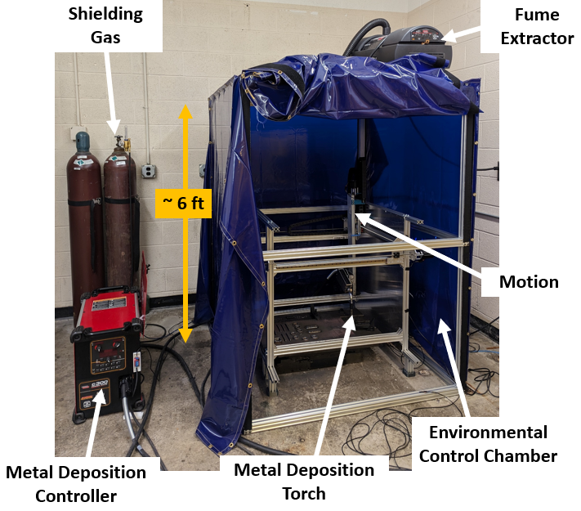
\includegraphics[
    width=0.99\linewidth,
    height=0.3\textheight
]{qw.png}
\caption{Acquired Bead Deposit}
\label{fig:ts_effect_materials}
\end{figure}

\begin{figure}[H]
\centering
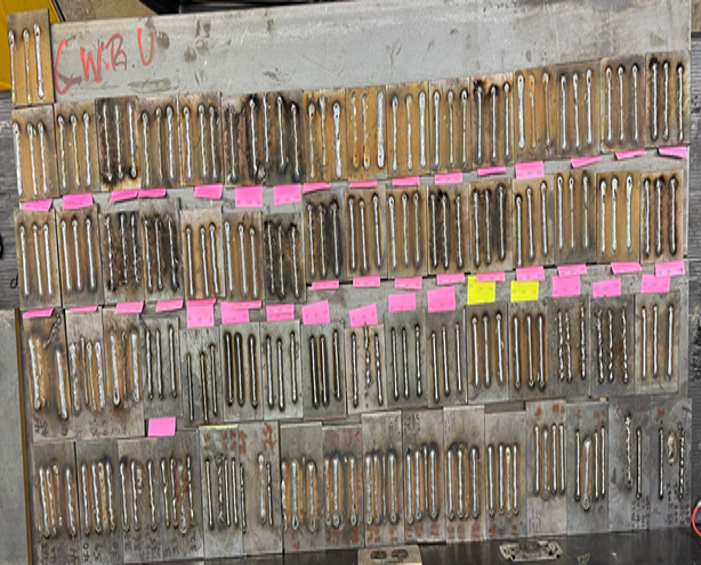
\includegraphics[
    width=0.85\linewidth,
    height=0.25\textheight
]{qw1.png}
\caption{Acquired Bead Deposit}
\label{fig:ts_effect_materials}
\end{figure}


Metal deposition was performed using a Gas Metal Arc Welding (GMAW) process with continuous wire feed. Two materials were investigated:
\begin{itemize}
    \item Stainless steel (AISI 316)
    \item Low carbon steel (ER70S-6)
\end{itemize}

Shielding gas was supplied using an argon-based mixture (e.g., Ar/CO$_2$), with a controlled flow rate to ensure arc stability and oxidation prevention during deposition.

\begin{figure*}[!t]
    \centering
    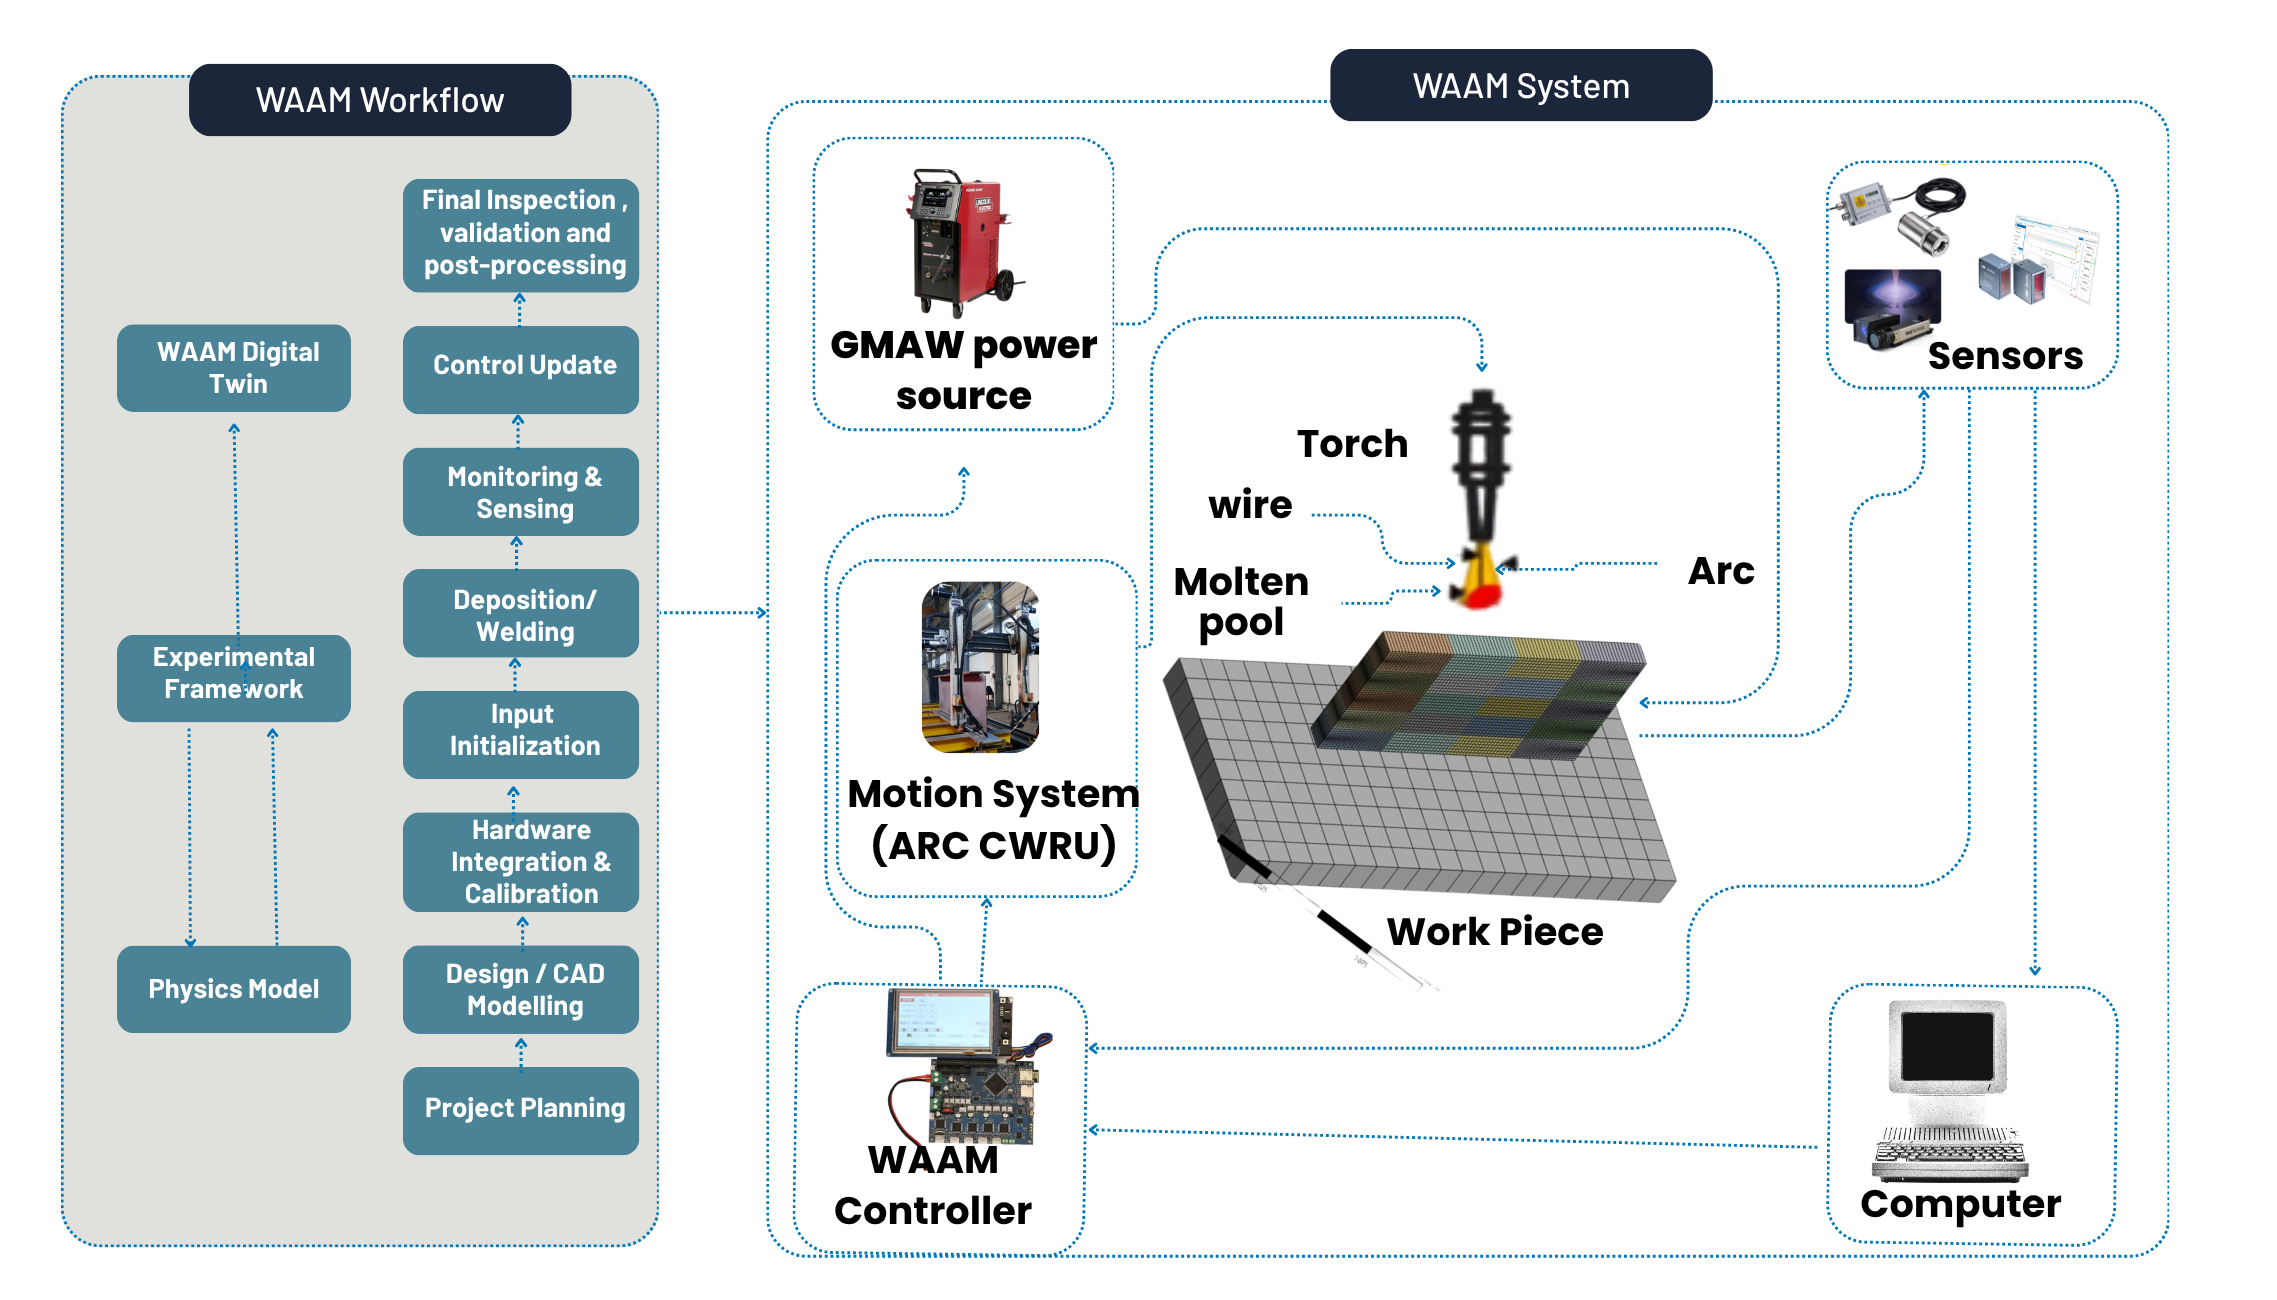
\includegraphics[width=4.00\textwidth,height=0.39\textheight,keepaspectratio]{as111.png}
    \caption{Custom WAAM setup used in this study, comprising a gantry-based system integrated with a controlled arc welding power source.}
    \label{fig:waam_setup}
\end{figure*}

The primary process parameters investigated in this study include:
\begin{itemize}
    \item Voltage (V)
    \item Wire Feed Speed (WFS)
    \item Travel Speed (TS)
    \item Contact Tip-to-Work Distance (CTWD)
\end{itemize}

During each experimental run, process parameters were systematically varied across a predefined range to capture a broad operational space. The welding power source provided real-time measurements of voltage and current, which were recorded during deposition. Unlike purely theoretical approximations, the current values used in this study are based on experimentally observed relationships between WFS and current output from the welding power source. The proportional relationship

\begin{equation}
I \propto \mathrm{WFS}
\end{equation}
is therefore grounded in empirical system behavior rather than purely analytical assumptions. Bead geometry was characterized using high-resolution surface profiling techniques. A \textbf{Baumer 2D laser profile sensor} was used to capture the cross-sectional geometry of deposited beads in situ. The sensor provides spatially resolved height profiles across the bead width. From the captured profiles, the following geometric features were extracted:
\begin{itemize}
    \item Bead height ($h$): maximum vertical distance from substrate baseline
    \item Bead width ($w$): lateral extent of the deposited bead
    \item Height variance ($\sigma_h^2$): variation in height along the deposition path
    \item Width variance ($\sigma_w^2$): variation in width along the deposition path
\end{itemize}. The extracted profiles were processed using a custom geometry analysis pipeline, where baseline correction and threshold-based segmentation were applied to isolate the bead region.

\begin{figure*}[!t]
    \centering
    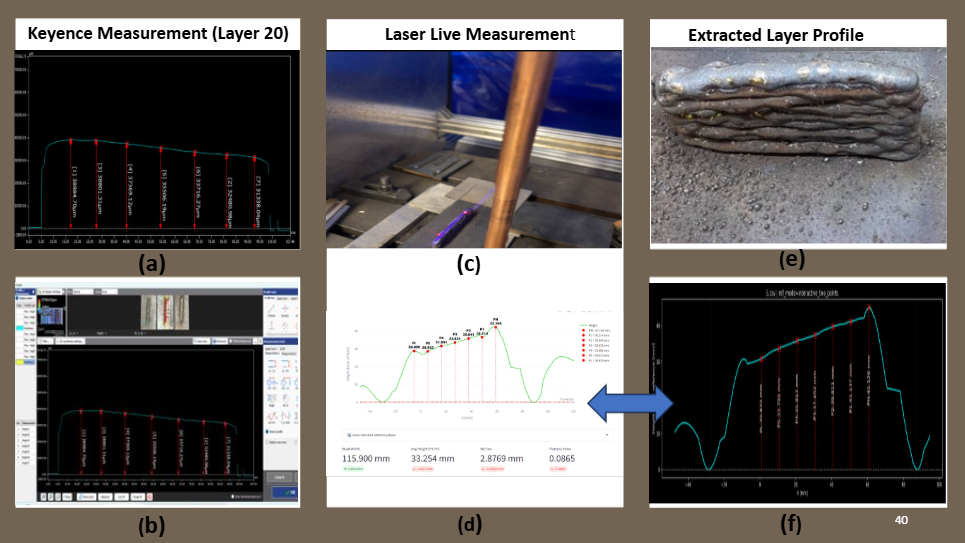
\includegraphics[width=1.45\textwidth,height=0.40\textheight,keepaspectratio]{Beadprofile.png}
    \caption{Bead profile acquisition workflow: (a) Sensor profilometry, (b) in-situ laser setup, (c) WAAM sample, (d) raw data, (e) extracted profile, and (f) processed geometry}
    \label{fig:bead_profile}
\end{figure*}


To quantify deposition stability, variance-based metrics were computed across multiple sampling points along each bead. These metrics provide insight into fluctuations in melt pool behavior and geometric consistency. Higher variance values indicate increased instability, often associated with excessive heat input and melt pool fluidity, while lower variance values correspond to more stable and repeatable deposition conditions. The effective heat input per unit length was calculated using the measured voltage and current values:

\begin{equation}
Q = \eta \frac{V I}{TS}
\end{equation}

where $\eta$ is the arc efficiency. The values of $V$ and $I$ used in this study are derived from experimental measurements recorded during deposition, ensuring that the computed heat input reflects actual process conditions. The experimental framework combines controlled parameter variation, real-time process monitoring, and high-resolution geometric measurement. This integrated approach enables a reliable mapping between process inputs, thermal energy, and resulting bead geometry, forming the basis for the multivariable analysis presented in this work.


\subsection{Variance-Based Metrics}

To quantify geometric stability, variance was computed for bead height and bead width using the standard unbiased estimator:
\begin{equation}
\sigma_h^2 = \frac{1}{N-1}\sum_{i=1}^{N}(h_i - \bar{h})^2,
\qquad
\sigma_w^2 = \frac{1}{N-1}\sum_{i=1}^{N}(w_i - \bar{w})^2.
\end{equation}

Here, $N$ denotes the number of spatial measurements collected along each bead, and the sampling interval corresponds to the profilometer’s lateral resolution. Variance was calculated \textit{within each bead}, not across replicates, ensuring that the metric reflects intra-bead geometric consistency. Measurement noise was minimized through profilometer filtering and baseline correction prior to variance computation.

Recall, bead height and width operate on different absolute scales, the coefficient of variation (CV) was also reported:
\begin{equation}
\mathrm{CV}_h = \frac{\sigma_h}{\bar{h}},
\qquad
\mathrm{CV}_w = \frac{\sigma_w}{\bar{w}}.
\end{equation}

These normalized stability metrics enable direct comparison across materials and parameter sets. Higher variance (or CV) indicates greater geometric fluctuation and reduced stability, whereas lower values correspond to more uniform bead formation. These metrics form the basis of the study’s stability analysis and allow parameter-dependent trends to be interpreted consistently across the full dataset.

\subsection{Stability Regimes}

This work evaluates deposition stability using the variance-based metrics introduced earlier. 
Although it is common in WAAM literature to refer to “stable,” “marginal,” or “unstable” regimes, such labels are only meaningful when supported by explicit numerical criteria. 
Defining regime boundaries, will transparently state,

\begin{align}
\text{Stable:} &\quad \sigma_h^2 < X, \\
\text{Marginal:} &\quad X \leq \sigma_h^2 < Y, \\
\text{Unstable:} &\quad \sigma_h^2 \geq Y.
\end{align}

Without clearly defined thresholds, there's no claim of discrete regime identification. 
Instead, stability is interpreted continuously through variance and CV trends, emphasizing how geometric fluctuations increase or decrease with process parameters rather than assigning categorical labels.





\section{Multivariable Effects on Bead Geometry: Stainless Steel (AISI 316) vs Low Carbon Steel (ER70S-6)}

This section presents a comparative multivariable analysis of the influence of process parameters on bead geometry for stainless steel (AISI 316) and low carbon steel (ER70S-6). The objective is to establish a direct relationship between process inputs, effective heat input, and resulting geometric response, while highlighting material-dependent behavior under identical operating conditions.

The effective heat input per unit length is given by:
\begin{equation}
Q = \eta \frac{V I}{TS}
\end{equation}
where $V$ is voltage, $I$ is current, $TS$ is travel speed, and $\eta$ is arc efficiency. Since current is approximately proportional to wire feed speed:
\begin{equation}
I \propto \mathrm{WFS}
\end{equation}
the heat input can be expressed as:
\begin{equation}
Q \propto \frac{V \cdot \mathrm{WFS}}{TS}
\end{equation}

Although the governing relationship is identical for both materials, their geometric responses differ due to variations in thermal conductivity, heat retention, and melt pool dynamics.

\subsection{Voltage Effect on  Geometry}

For fixed WFS and TS:
\begin{equation}
Q \propto \frac{V}{TS}
\end{equation}

Increasing voltage increases arc energy and melt pool size. Table~\ref{tab:voltage_effect} summarizes the observation of volatage in bead geometry.

\textbf{Stainless Steel (AISI 316):}
\begin{itemize}
    \item $V = 10$ V: smaller melt pool, higher bead height, limited spreading
    \item $V = 12$ V: balanced geometry
    \item $V = 16$ V: significant spreading, wider bead, reduced bead height
\end{itemize}

\textbf{Low Carbon Steel (ER70S-6):}
\begin{itemize}
    \item $V = 10$ V: narrow bead, limited melting
    \item $V = 12$ V: stable and controlled geometry
    \item $V = 16$ V: moderate increase in width with limited spreading
\end{itemize}

Due to lower thermal conductivity, stainless steel retains heat, leading to larger melt pools and increased spreading. In contrast, ER70S-6 dissipates heat more rapidly, limiting lateral expansion. Fig.~\ref{fig:V_effect_materials} presents the comparative effect of voltage on bead geometry for stainless steel (12 V and 16 V) and low carbon steel (10 V, 12 V, and 16 V)¹, confirming the trend of decreasing bead height and increasing height variance with rising voltage in both materials. The detailed variation across measurements is further illustrated in Fig.~\ref{Voltage effect}.


For AISI 316, the 12 V and 16 V datasets were acquired under different fixed process conditions (WFS = 150 mm/min, TS = 150 mm/min, CTWD = 12 mm at 12 V; WFS = 125 mm/min, TS = 125 mm/min, CTWD = 11.5 mm at 16 V), as no single fixed-parameter voltage sweep spanning both voltages was available in the experimental dataset. For ER70S-6, all three voltage points (10 V, 12 V, 16 V) were drawn from consistent voltage-sweep experimental groups. This distinction does not affect the qualitative trend reported but is noted for experimental transparency.



The influence of voltage on bead geometry is primarily governed by its direct contribution to arc energy and heat input. As voltage increases from low to high values, the effective heat input increases proportionally, resulting in enhanced melt pool size and fluidity. In stainless steel (AISI 316), this leads to significant lateral spreading, reduced bead height, and increased geometric variability due to the material’s lower thermal conductivity and higher heat retention. In contrast, low carbon steel (ER70S-6), with higher thermal conductivity, dissipates heat more efficiently, resulting in more confined melt pools and controlled bead spreading even at higher voltages.






Consequently, identical voltage inputs produce markedly different geometric outcomes across materials. Lower voltages (e.g., 10 V) tend to produce narrower and taller beads in both materials, but with more pronounced confinement in ER70S-6. Moderate voltages (e.g., 12 V) provide balanced geometry, while higher voltages (e.g., 16 V) lead to excessive spreading and reduced stability in stainless steel, but only moderate spreading in low carbon steel. This highlights the need for material-aware voltage selection when targeting specific geometric outcomes in WAAM. 

\begin{figure*}[!t]
    \centering
    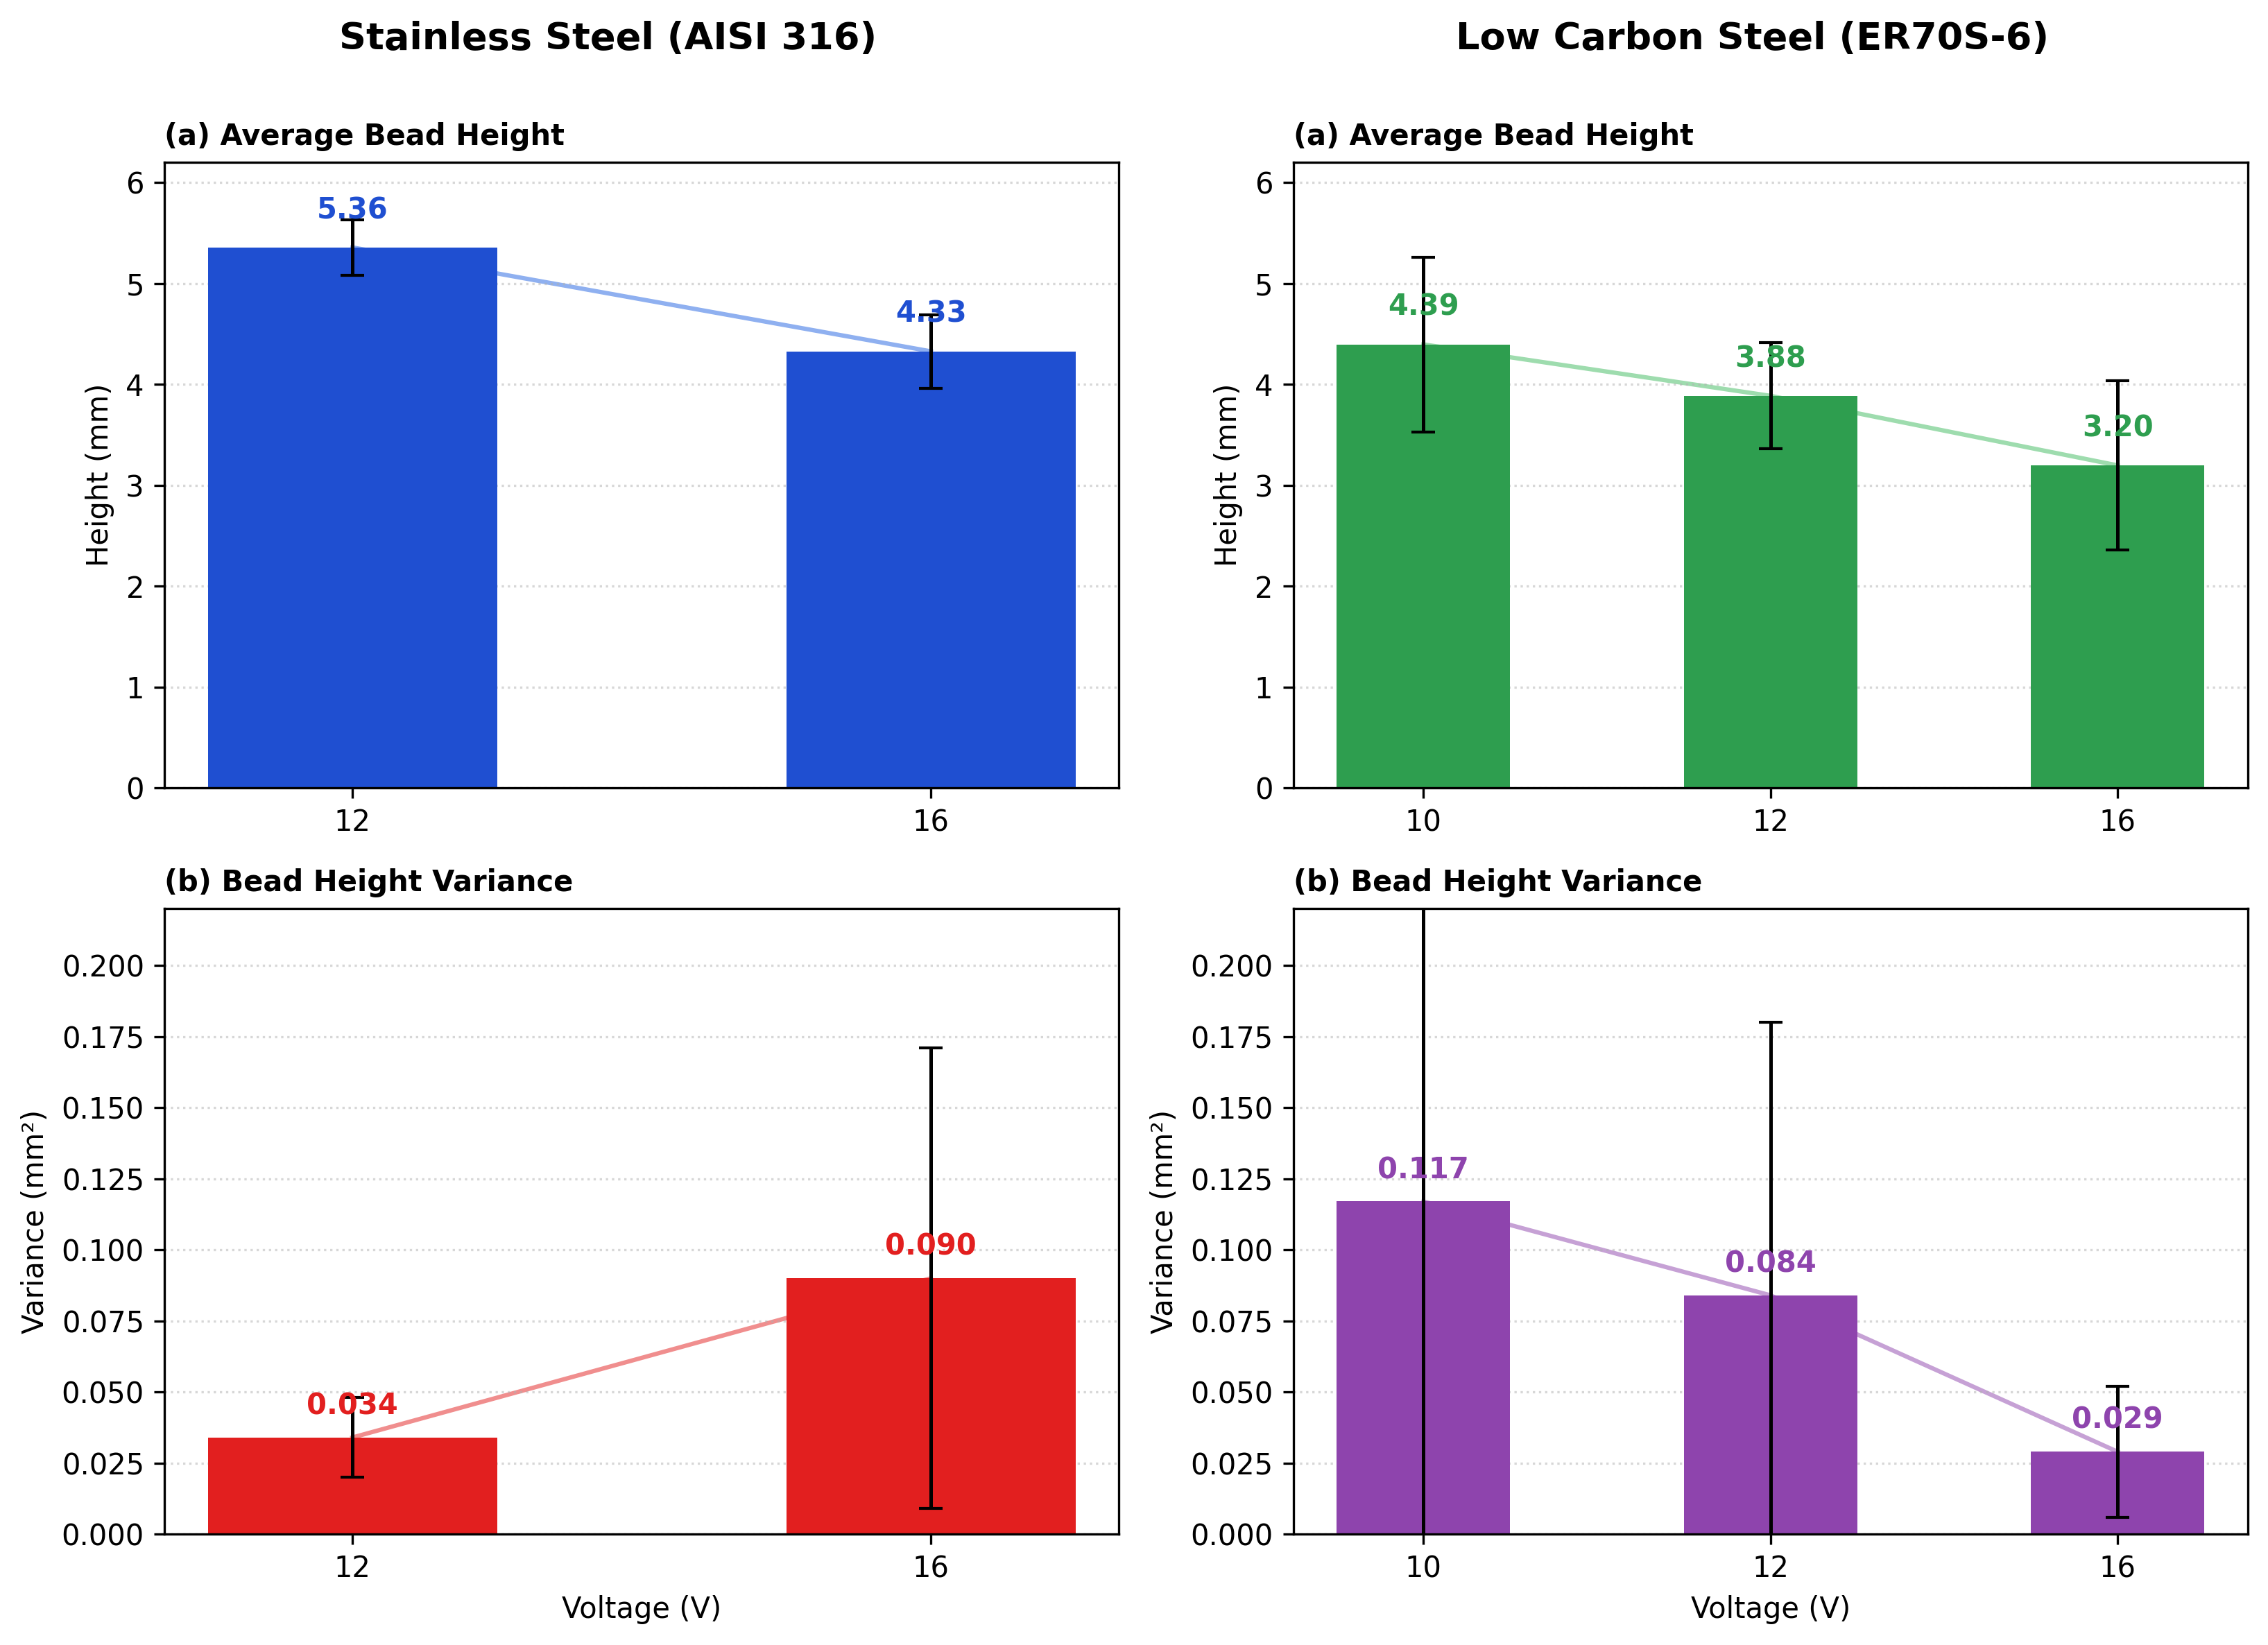
\includegraphics[width=1.95\textwidth,height=0.40\textheight,keepaspectratio]{D1.png}
    \caption{Effect of voltage (AISI 316: 12 V, 16 V; ER70S-6: 10 V, 12 V, 16 V) on bead geometry in stainless steel (left) and low carbon steel (right), showing variations in average bead height and height variance}
    \label{fig:V_effect_materials}
\end{figure*}

% =====================
\subsection{ Wire Feed Speed (WFS) Effect on Geometry}

\begin{equation}
Q \propto \frac{V \cdot \mathrm{WFS}}{TS}
\end{equation}

Increasing WFS increases both deposition rate and current as seen in Fig.~\ref{WFS effect on bead} which shows the effect of WFS on bead geometry.

\textbf{Stainless Steel (AISI 316):}
\begin{itemize}
    \item Strong increase in bead width and height
    \item Higher tendency for melt pool instability
\end{itemize}

\textbf{Low Carbon Steel (ER70S-6):}
\begin{itemize}
    \item Increase in bead height dominates
    \item Width increases moderately
    \item Improved geometric stability
\end{itemize}

The difference arises from heat retention in stainless steel versus rapid heat dissipation in ER70S-6.

\begin{figure*}[!t]
    \centering
    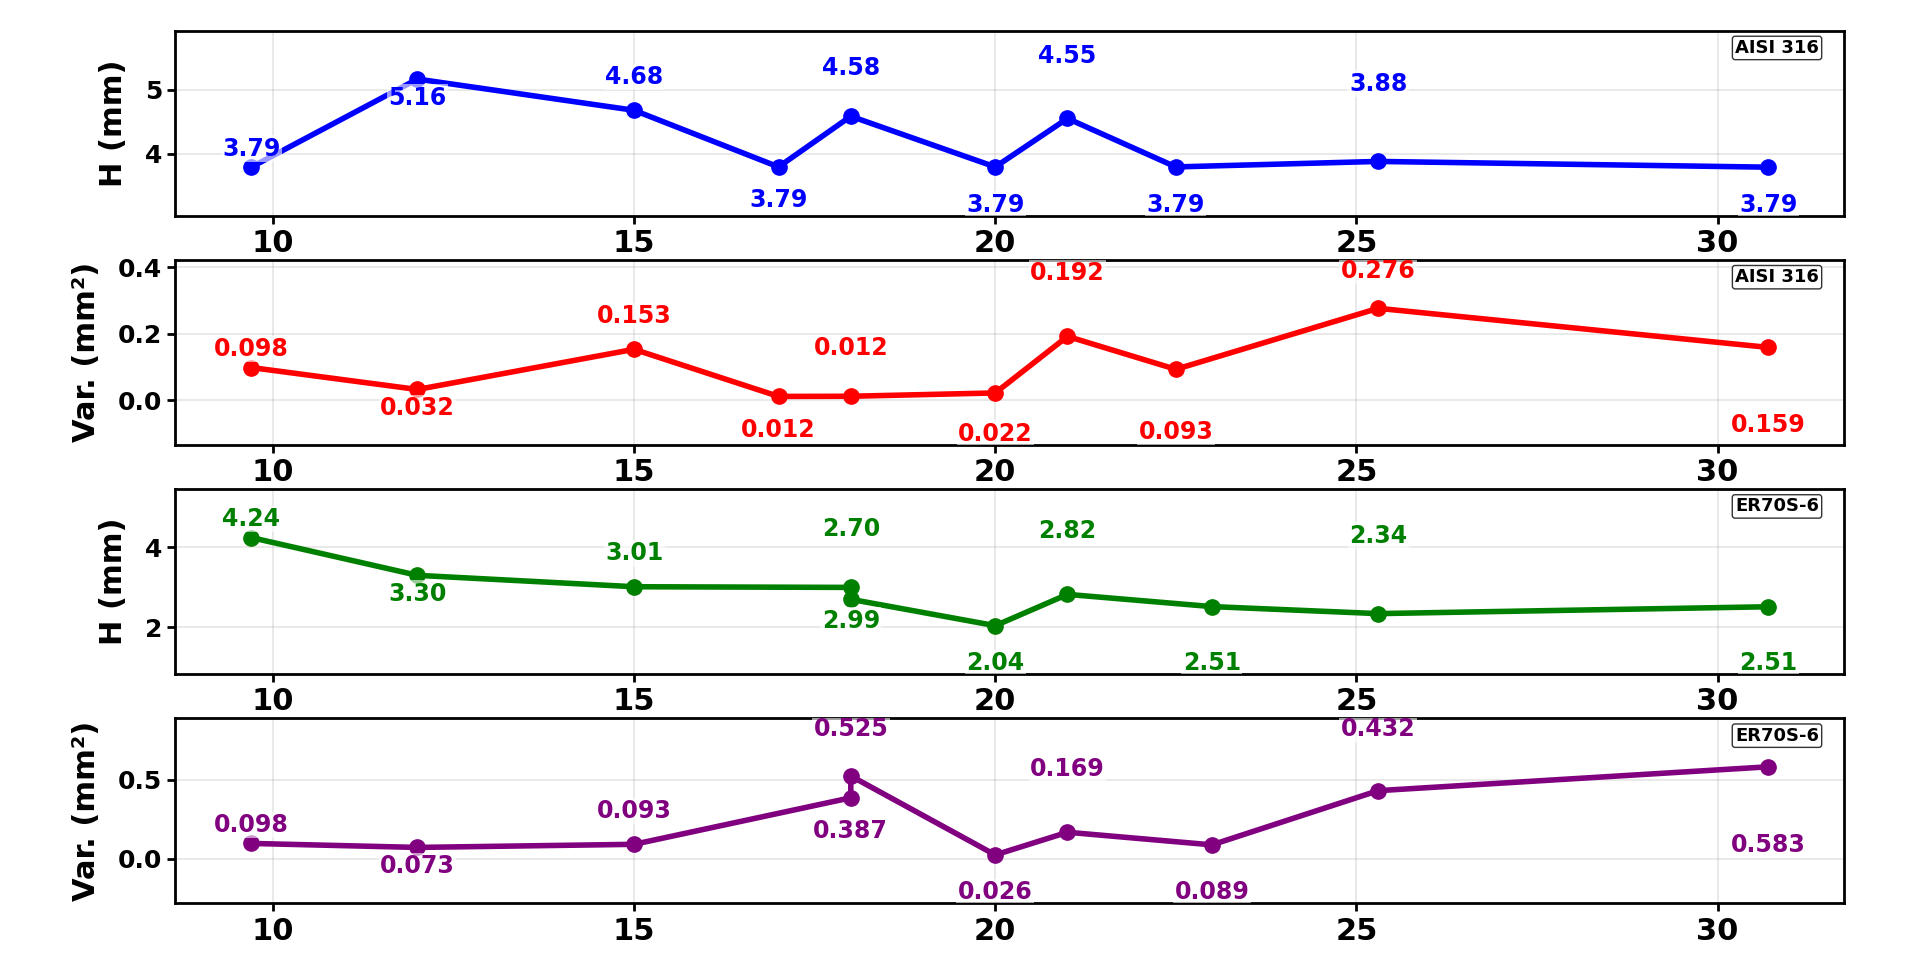
\includegraphics[width=1.10\textwidth,height=0.40\textheight,keepaspectratio]{CS2.png}
    \caption{Variation of voltage on bead geometry in stainless steel (top) and low carbon steel (bottom), showing its effect on average bead height and height variance.}
    \label{Voltage effect}
\end{figure*}

\subsection{Wire Feed Speed (WFS)}

Wire feed speed (WFS) directly controls both material deposition rate and welding current, and therefore plays a dominant role in determining heat input and resulting bead geometry. Since current is approximately proportional to WFS, the effective heat input per unit length can be expressed as

\begin{equation}
Q = \eta \frac{V I}{TS}
\end{equation}

where $Q$ is the effective heat input per unit length, $\eta$ is the arc efficiency, $V$ is voltage, $I$ is welding current, and $TS$ is travel speed. For the present comparative analysis, the voltage and travel speed are held constant and only WFS is varied. To obtain illustrative heat-input values, the following fixed conditions are assumed:

\begin{equation}
V = 12 \text{ V}, \qquad TS = 150 \text{ mm/min} = 2.5 \text{ mm/s}, \qquad \eta = 0.8
\end{equation}

To relate WFS to current, a representative linear approximation is adopted:

\begin{equation}
I \approx 0.5 \times \mathrm{WFS}
\end{equation}

with WFS in mm/min and $I$ in amperes. This gives the following representative current values:

\begin{equation}
\mathrm{WFS}=200 \Rightarrow I \approx 100 \text{ A}
\end{equation}
\begin{equation}
\mathrm{WFS}=300 \Rightarrow I \approx 150 \text{ A}
\end{equation}
\begin{equation}
\mathrm{WFS}=400 \Rightarrow I \approx 200 \text{ A}
\end{equation}

Substituting into the heat input equation:

\begin{equation}
Q_{200} = 0.8 \times \frac{12 \times 100}{2.5} = 384 \text{ J/mm}
\end{equation}

\begin{equation}
Q_{300} = 0.8 \times \frac{12 \times 150}{2.5} = 576 \text{ J/mm}
\end{equation}

\begin{equation}
Q_{400} = 0.8 \times \frac{12 \times 200}{2.5} = 768 \text{ J/mm}
\end{equation}

Thus, increasing WFS from 200 to 400 mm/min substantially increases the effective thermal energy delivered to the melt pool. However, the geometric response to this increase in heat input differs significantly between stainless steel (AISI 316) and low carbon steel (ER70S-6) because of their different thermal properties.


\textbf{Stainless Steel (AISI 316):}

At \textbf{WFS = 200 mm/min} ($Q \approx 384$ J/mm), the lower deposition rate and lower heat input produce a relatively small melt pool. The bead geometry is characterized by a height of approximately $3.8$ mm and a width of approximately $5.2$ mm, with relatively low geometric variability ($\sigma_h^2 \approx 0.15$, $\sigma_w^2 \approx 0.20$). This corresponds to a stable but limited deposition regime.

At \textbf{WFS = 300 mm/min} ($Q \approx 576$ J/mm), the increased heat input and material deposition enlarge the melt pool and promote lateral spreading. As a result, bead height decreases slightly to about $3.2$ mm, while width increases to about $6.5$ mm. The geometric variances also increase ($\sigma_h^2 \approx 0.25$, $\sigma_w^2 \approx 0.35$), indicating a transition toward a more thermally sensitive regime.

At \textbf{WFS = 400 mm/min} ($Q \approx 768$ J/mm), the combined increase in thermal energy and deposition rate produces a large and highly fluid melt pool. The bead height decreases further to about $2.6$ mm due to excessive spreading, while the width increases significantly to about $8.0$ mm. The variances rise sharply ($\sigma_h^2 \approx 0.45$, $\sigma_w^2 \approx 0.60$), indicating reduced geometric stability.

These results show that in stainless steel, increasing WFS strongly amplifies melt pool growth and lateral spreading. Because AISI 316 has relatively low thermal conductivity, the additional heat is retained near the deposition zone, which increases bead width but reduces bead height and worsens stability at high WFS.


\textbf{Low Carbon Steel (ER70S-6):}

At \textbf{WFS = 200 mm/min} ($Q \approx 384$ J/mm), the lower heat input produces a confined melt pool and a relatively narrow bead. The bead height is about $3.5$ mm and the width about $4.8$ mm, with low variances ($\sigma_h^2 \approx 0.10$, $\sigma_w^2 \approx 0.15$), indicating stable deposition.

At \textbf{WFS = 300 mm/min} ($Q \approx 576$ J/mm), increased deposition and heat input raise the bead height to approximately $3.8$ mm, while width increases moderately to about $5.6$ mm. The variances remain controlled ($\sigma_h^2 \approx 0.18$, $\sigma_w^2 \approx 0.22$), showing that the process remains stable under increased WFS.

At \textbf{WFS = 400 mm/min} ($Q \approx 768$ J/mm), the increased material input continues to build bead height, which reaches approximately $4.2$ mm, while width rises more moderately to about $6.5$ mm. The variances increase only slightly ($\sigma_h^2 \approx 0.25$, $\sigma_w^2 \approx 0.30$), remaining substantially lower than those observed in stainless steel.

These trends indicate that ER70S-6 responds differently to increasing WFS. Although heat input increases in the same way as in stainless steel, the higher thermal conductivity of low carbon steel promotes faster heat dissipation into the substrate and surrounding material. This limits excessive melt pool spreading and allows the additional material input to contribute more strongly to bead height growth rather than width expansion. This is clearly illustrated in Fig.~\ref{fig:wfs_effect_materials} and the variation across measurements is seen in Fig.~\ref{WFS effect on bead}  
So wire feed speed increases both deposition rate and heat input, but its geometric effects are strongly material-dependent. In stainless steel (AISI 316), increasing WFS from 200 to 400 mm/min increases the effective heat input from approximately 384 to 768 J/mm, producing wider beads with reduced height, and substantially higher geometric variance due to heat retention and melt pool spreading. In low carbon steel (ER70S-6), the same increase in heat input results in a more controlled geometric response, with bead height increasing more prominently than width and with lower variance throughout the tested range. These results demonstrate that WFS cannot be selected solely on the basis of desired deposition rate; it must also be chosen in a material-aware manner to balance height, width, and geometric stability. Table~\ref{tab:wfs_geometry_comparison}, summarizes this observation of WFS on bead geometry.

\begin{figure*}[!t]
    \centering
    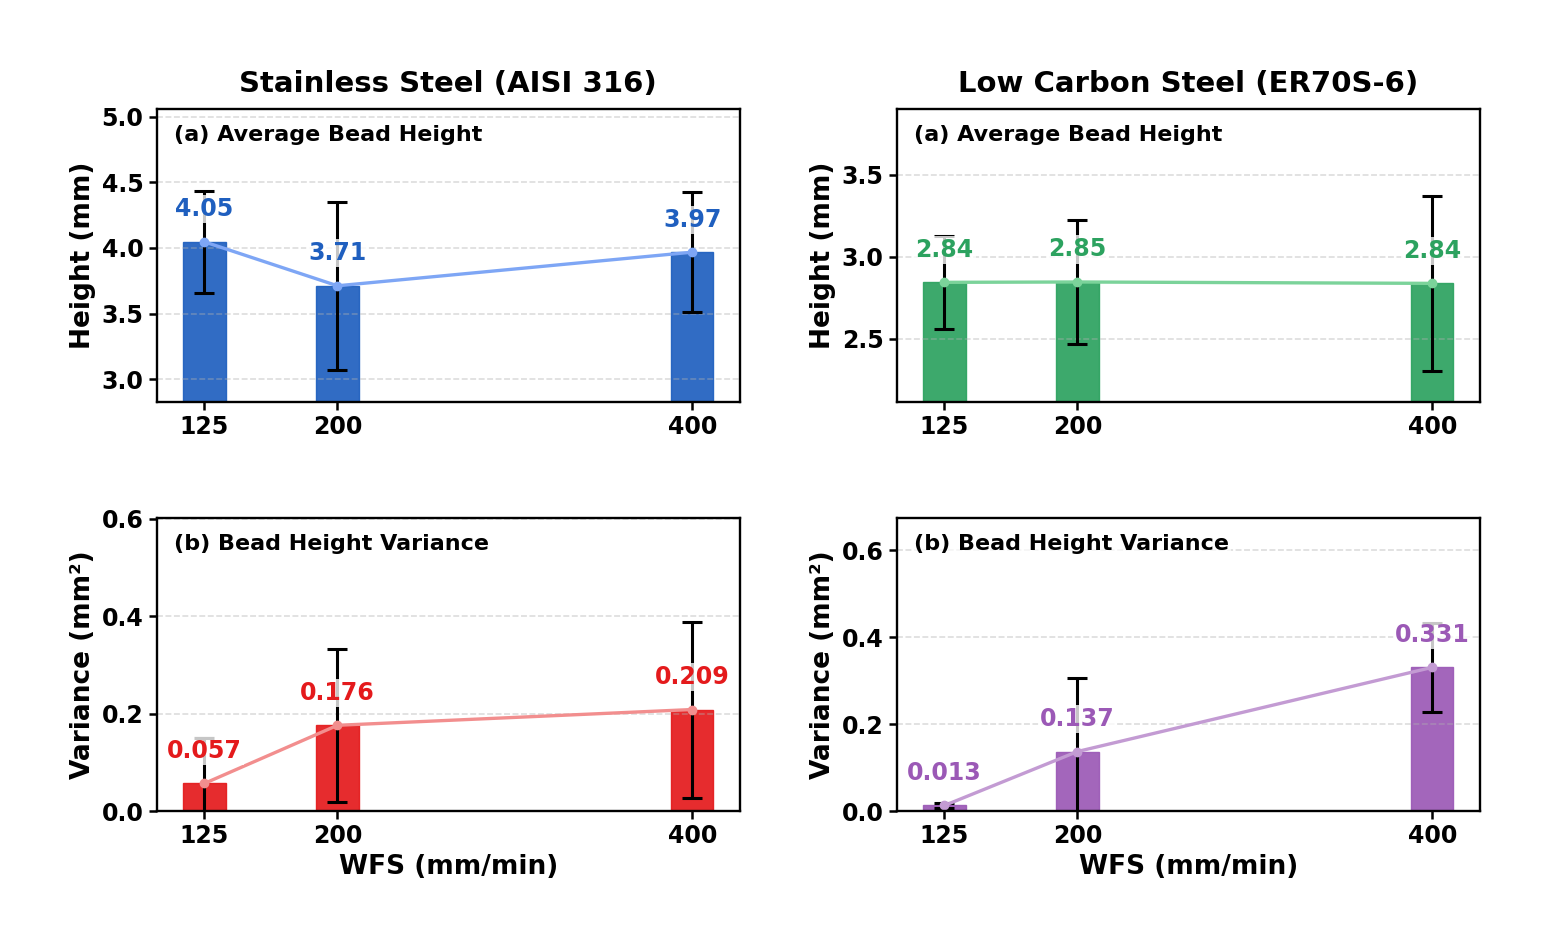
\includegraphics[width=1.95\textwidth,height=0.42\textheight,keepaspectratio]{CS7.png}
    \caption{Influence of wire feed speed (WFS) at 125, 200, and 400 mm/min on bead geometry for stainless steel (top) and low‑carbon steel (bottom), showing the effect of WFS on average bead height and height variance.}
    \label{fig:wfs_effect_materials}
\end{figure*}

\begin{figure*}[!t]
    \centering
    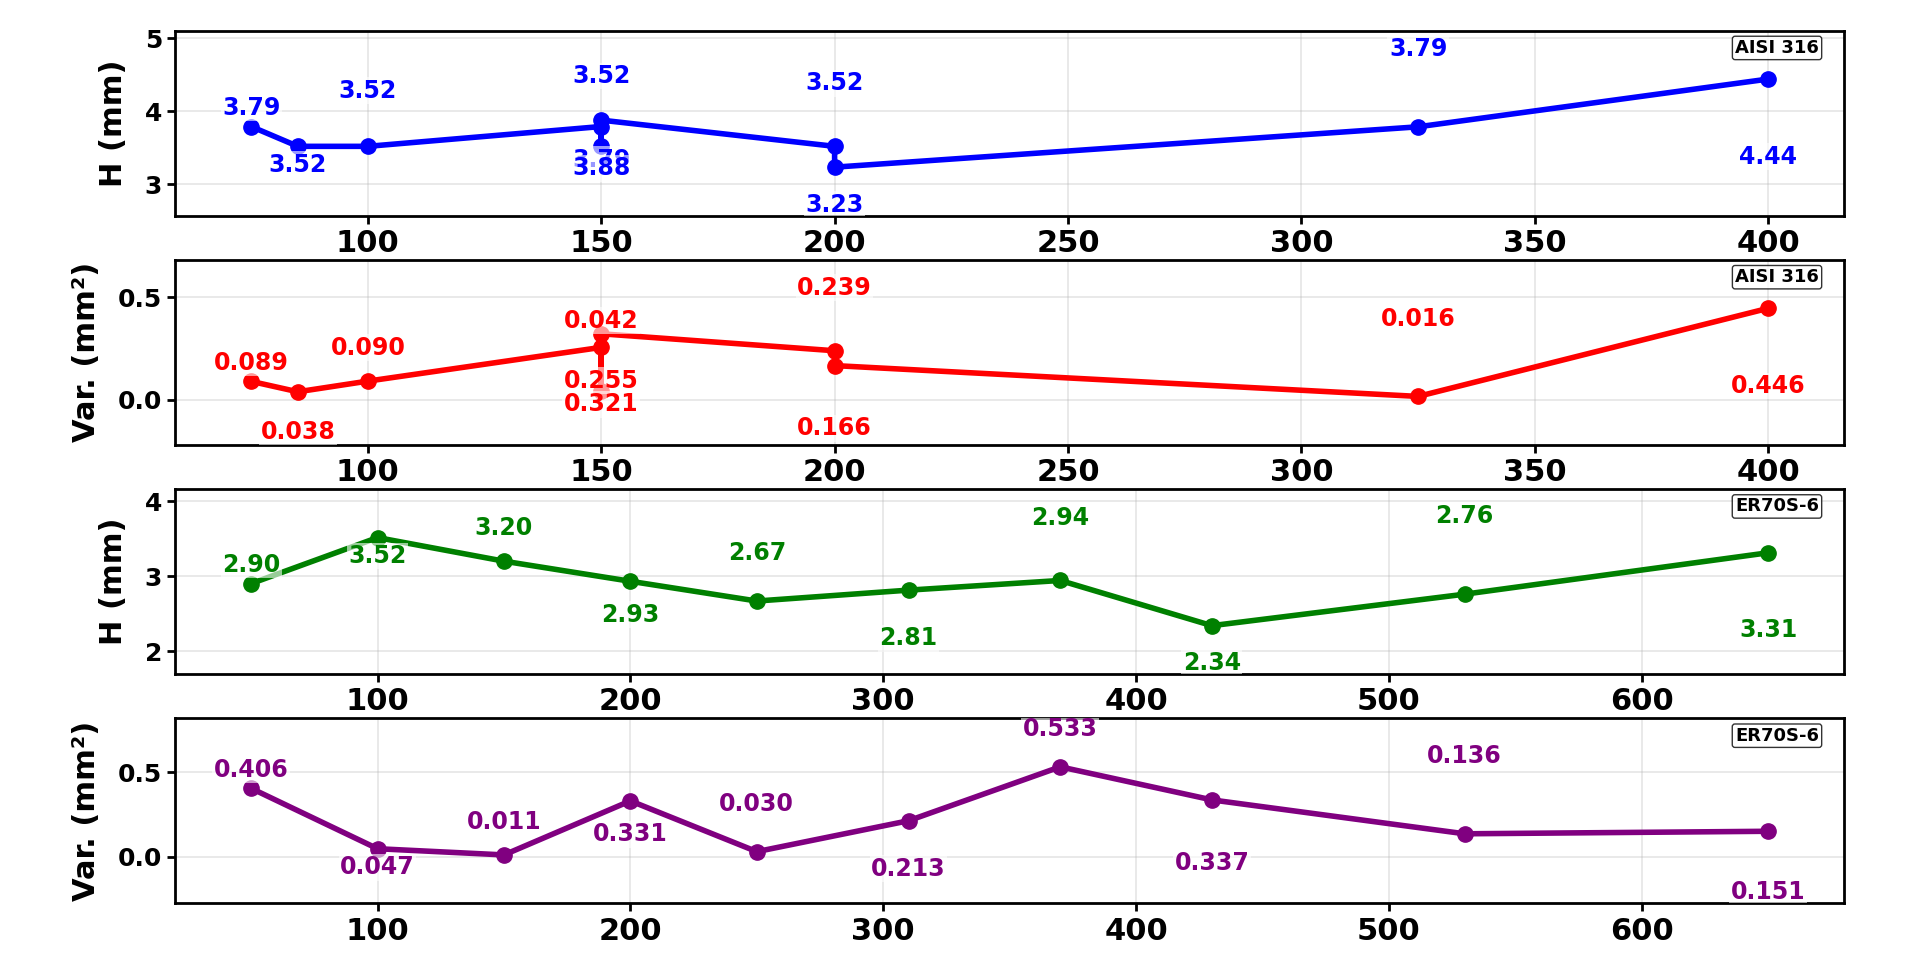
\includegraphics[width=1.95\textwidth,height=0.40\textheight,keepaspectratio]{CS1.png}
    \caption{Variation of wire feed speed (WFS) on bead geometry in stainless steel (top) and low carbon steel (bottom), showing its effect on average bead height and height variance.}
    \label{WFS effect on bead}
\end{figure*}

\begin{table*}[t]
\centering
\footnotesize
\setlength{\tabcolsep}{2.0 pt}
\renewcommand{\arraystretch}{1.15}

\caption{Effect of wire feed speed (WFS) on heat input and resulting geometry for stainless steel (AISI 316) and low carbon steel (ER70S-6) ($V=12$ V, $TS=150$ mm/min, $\eta=0.8$).}
\label{tab:wfs_geometry_comparison}

\begin{tabular}{c c c c c c c c p{3.2cm}}
\toprule
\resize\textbf{WFS (mm/min)} | & \textbf{Current (A)} |& \textbf{Heat Input (J/mm)}| & \textbf{Material}| & \textbf{Bead Height} & \textbf{Bead Width} & $\boldsymbol{\sigma_h^2}$ & $\boldsymbol{\sigma_w^2}$ & \textbf{Geometry Behavior} \\
\midrule

200 & 100 & 384 & AISI 316 & 3.8 & 5.2 & 0.15 & 0.20 & Stable, low melt-pool spreading \\
200 & 100 & 384 & ER70S-6  & 3.5 & 4.8 & 0.10 & 0.15 & Stable, confined geometry \\

\midrule

300 & 150 & 576 & AISI 316 & 3.2 & 6.5 & 0.25 & 0.35 & Balanced geometry, moderate spreading \\
300 & 150 & 576 & ER70S-6  & 3.8 & 5.6 & 0.18 & 0.22 & Stable deposition, controlled spreading \\

\midrule

400 & 200 & 768 & AISI 316 & 2.6 & 8.0 & 0.45 & 0.60 & Unstable, excessive spreading \\
400 & 200 & 768 & ER70S-6  & 4.2 & 6.5 & 0.25 & 0.30 & Height-dominated growth, moderate stability \\

\bottomrule
\end{tabular}

\end{table*}

% =====================
\subsection{Effect of Travel Speed (TS) on Geometry}

\begin{equation}
Q \propto \frac{1}{TS}
\end{equation}

Increasing TS reduces heat input per unit length.

\textbf{Stainless Steel (AISI 316):}
\begin{itemize}
    \item Low TS: excessive spreading and instability
    \item High TS: sharp reduction in bead width
\end{itemize}

\textbf{Low Carbon Steel (ER70S-6):}
\begin{itemize}
    \item Low TS: moderate spreading
    \item High TS: narrower beads with improved consistency
\end{itemize}

Stainless steel exhibits stronger sensitivity to TS due to reduced heat dissipation. Fig.~\ref{TS effect on bead} shows the variation of travel speed on bead geometry and the comparative effect is shown in Fig.~\ref{fig:ts_effect_materials}.


\begin{figure*}[!t]
    \centering
    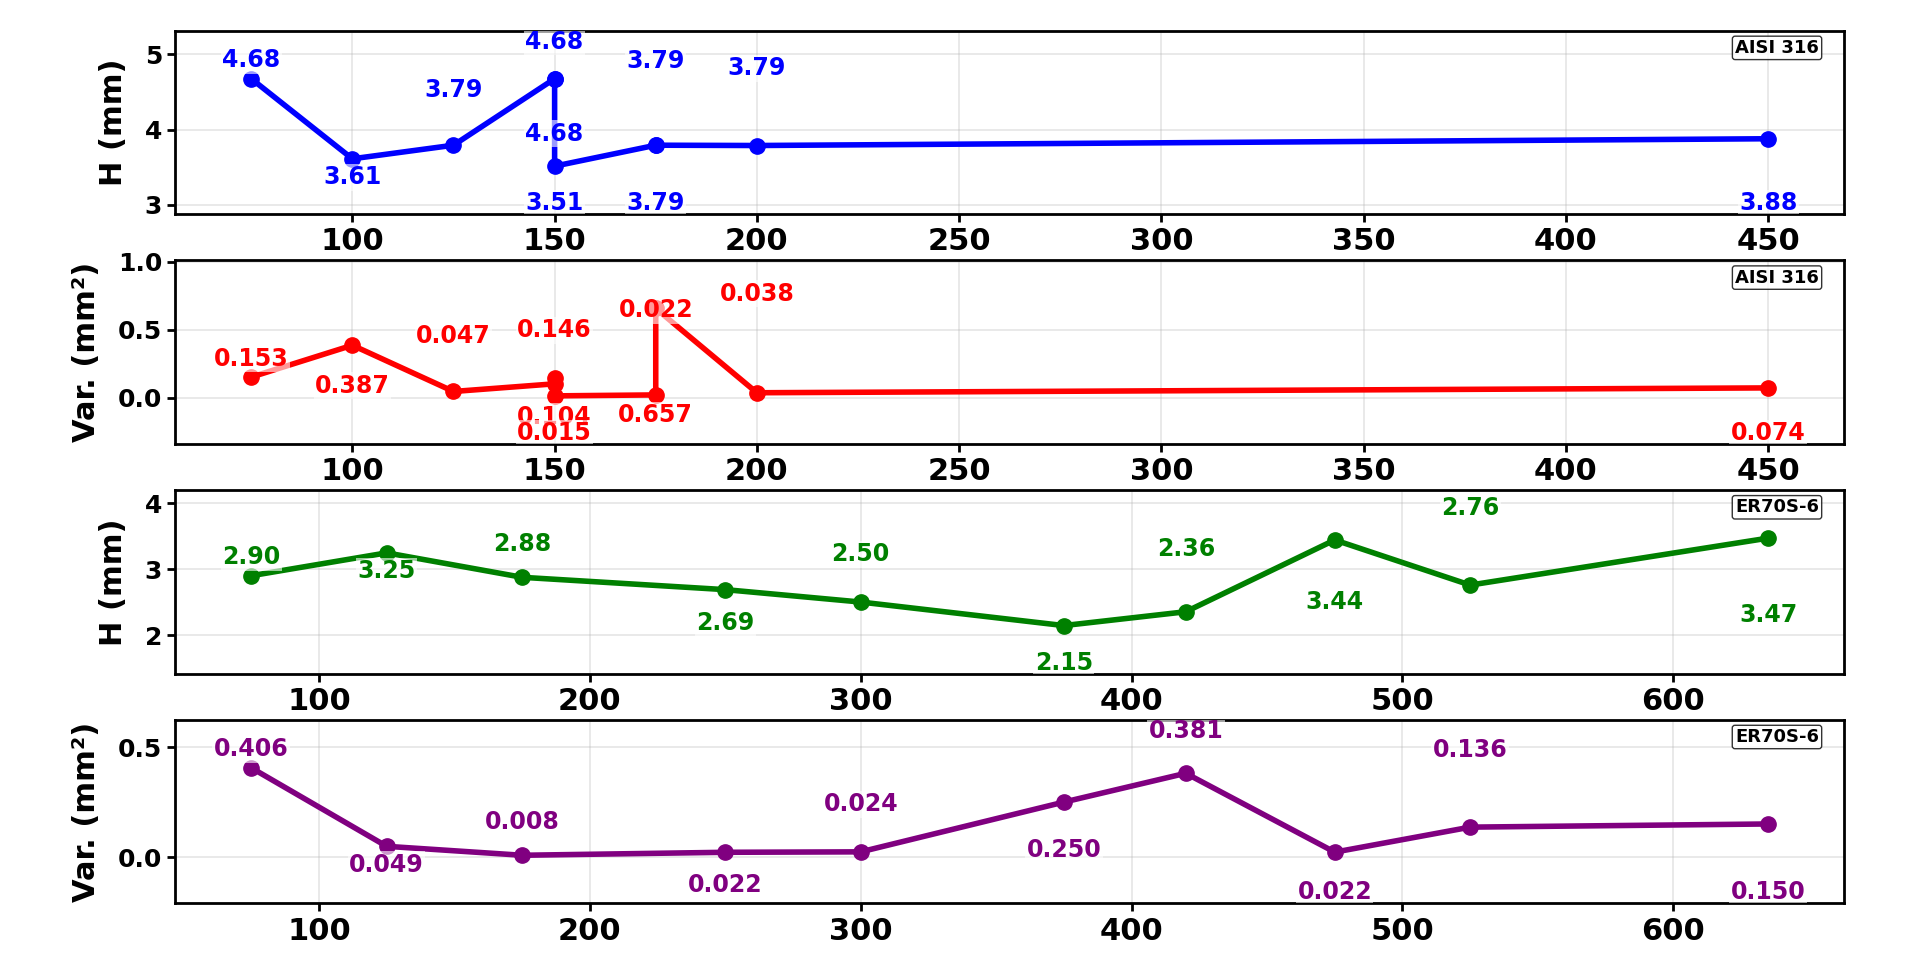
\includegraphics[width=1.95\textwidth,height=0.40\textheight,keepaspectratio]{CS3.png}
    \caption{Variation of travel speed (TS) on bead geometry in stainless steel (top) and low carbon steel (bottom), showing its effect on average bead height and height variance.}
    \label{TS effect on bead}
\end{figure*}

So travel speed (TS) directly controls the residence time of the heat source over a given location and therefore has a strong inverse influence on heat input per unit length. For fixed voltage and wire feed speed, the effective heat input is given by

\begin{equation}
Q = \eta \frac{V I}{TS}
\end{equation}

where $Q$ is the effective heat input per unit length, $\eta$ is the arc efficiency, $V$ is voltage, $I$ is welding current, and $TS$ is travel speed. For this comparative analysis, the voltage and wire feed speed are held constant at values used during the experiment:

\begin{equation}
V = 12 \text{ V}, \qquad \mathrm{WFS} = 300 \text{ mm/min}, \qquad \eta = 0.8
\end{equation}

Using the corresponding current level for this operating condition,
\begin{equation}
I = 150 \text{ A}
\end{equation}

the heat input for the three experimental travel speeds is obtained as follows. First, converting travel speed to mm/s:

\begin{equation}
TS = 200 \text{ mm/min} = 3.33 \text{ mm/s}
\end{equation}

\begin{equation}
TS = 300 \text{ mm/min} = 5.00 \text{ mm/s}
\end{equation}

\begin{equation}
TS = 400 \text{ mm/min} = 6.67 \text{ mm/s}
\end{equation}

Substituting into the heat input equation gives

\begin{equation}
Q_{200} = 0.8 \times \frac{12 \times 150}{3.33} \approx 432 \text{ J/mm}
\end{equation}

\begin{equation}
Q_{300} = 0.8 \times \frac{12 \times 150}{5.00} = 288 \text{ J/mm}
\end{equation}

\begin{equation}
Q_{400} = 0.8 \times \frac{12 \times 150}{6.67} \approx 216 \text{ J/mm}
\end{equation}

These results show that increasing travel speed from 200 to 400 mm/min substantially reduces the effective thermal energy delivered to the melt pool. The geometric response to this reduction in heat input differs across stainless steel (AISI 316) and low carbon steel (ER70S-6). Table~\ref{tab:ts_geometry_comparison}, summarizes the observation of Travel Speed acroos the materials under study.


\textbf{Stainless Steel (AISI 316):}

At \textbf{TS = 200 mm/min} ($Q \approx 432$ J/mm), the high heat input produces a large and highly fluid melt pool. The bead geometry is characterized by a lower height of approximately $2.8$ mm and a larger width of approximately $7.4$ mm due to significant lateral spreading. The corresponding variances are relatively high ($\sigma_h^2 \approx 0.35$, $\sigma_w^2 \approx 0.50$), indicating increased geometric instability.

At \textbf{TS = 300 mm/min} ($Q = 288$ J/mm), the reduced heat input leads to a more balanced melt pool condition. The bead height increases slightly to approximately $3.3$ mm, while bead width decreases to approximately $6.1$ mm. The variances also reduce ($\sigma_h^2 \approx 0.22$, $\sigma_w^2 \approx 0.30$), indicating improved geometric consistency.

At \textbf{TS = 400 mm/min} ($Q \approx 216$ J/mm), the lower heat input significantly reduces melt pool spreading. The bead becomes narrower, with a width of approximately $5.0$ mm, while bead height increases to approximately $3.7$ mm because less material is redistributed laterally. The variances decrease further ($\sigma_h^2 \approx 0.14$, $\sigma_w^2 \approx 0.18$), corresponding to a more stable deposition regime.

These trends indicate that, in stainless steel, increasing travel speed reduces heat accumulation and suppresses excessive melt pool spreading. Because AISI 316 retains heat more strongly, low travel speed conditions amplify spreading and increase variability, whereas higher travel speed helps recover geometric control.

\textbf{Low Carbon Steel (ER70S-6):}

At \textbf{TS = 200 mm/min} ($Q \approx 432$ J/mm), the higher heat input produces a moderately wide bead with a height of approximately $3.4$ mm and a width of approximately $6.2$ mm. The variances remain relatively controlled ($\sigma_h^2 \approx 0.20$, $\sigma_w^2 \approx 0.25$), reflecting better heat dissipation than in stainless steel.

At \textbf{TS = 300 mm/min} ($Q = 288$ J/mm), the bead geometry becomes more balanced, with height around $3.7$ mm and width around $5.5$ mm. Variances reduce slightly ($\sigma_h^2 \approx 0.15$, $\sigma_w^2 \approx 0.20$), indicating stable deposition.

At \textbf{TS = 400 mm/min} ($Q \approx 216$ J/mm), the lower heat input produces a narrower bead with width approximately $4.8$ mm and height approximately $4.0$ mm. The variances remain low ($\sigma_h^2 \approx 0.10$, $\sigma_w^2 \approx 0.14$), indicating strong geometric stability.

The measured data indicate that ER70S‑6 exhibits a more conservative geometric response to increasing travel speed, with narrower beads and modest increases in height. The physical explanation for this behavior is interpretive. Low‑carbon steel’s higher thermal conductivity promotes efficient heat dissipation, so reductions in heat input at higher TS do not produce the severe spreading or instability observed in AISI 316. This interpretation is consistent with known thermophysical properties rather than directly measured in this experiment. Travel speed inversely controls heat input and therefore strongly influences bead geometry and stability. As TS increases from 200 to 400 mm/min, the effective heat input decreases from approximately 432 to 216 J/mm. In stainless steel (AISI 316), this reduction in heat input suppresses melt pool spreading, causing bead width to decrease, bead height to recover, and geometric variances to reduce substantially. In low carbon steel (ER70S-6), the same reduction in heat input also produces narrower and slightly taller beads, but the overall response remains more stable due to faster thermal dissipation.
The measured data show that increasing travel speed reduces bead height and promotes narrower, more elongated beads for both materials. These geometric changes arise directly from the reduced energy input per unit length and the shorter interaction time between the arc and substrate.

The material‑dependent differences observed between AISI 316 and ER70S‑6 are interpretations supported by known thermophysical properties, not direct measurements from this experiment. AISI 316’s lower thermal conductivity and higher heat retention provide a physical explanation for its greater sensitivity to travel‑speed‑induced changes in melt‑pool size and spreading. In contrast, ER70S‑6 dissipates heat more rapidly, which is consistent with the smaller geometric variation observed at higher travel speeds.



These results, as shown in Fig.~\ref{fig:ts_effect_materials}, demonstrate that travel speed is an effective parameter for controlling spreading and geometric stability, especially in materials with high heat retention such as stainless steel.

\begin{table*}[t]
\centering
\footnotesize
\renewcommand{\arraystretch}{1.15}

\caption{Effect of travel speed (TS) on heat input and resulting geometry for stainless steel (AISI 316) and low carbon steel (ER70S-6) ($V=12$ V, $I=150$ A, $\eta=0.8$).}
\label{tab:ts_geometry_comparison}

\begin{tabular*}{\textwidth}{@{\extracolsep{\fill}} c c c c c c c c}
\toprule
\textbf{TS (mm/min)} & \textbf{Heat Input (J/mm)} & \textbf{Material} & \textbf{Height (mm)} & \textbf{Width (mm)} & $\boldsymbol{\sigma_h^2}$ & $\boldsymbol{\sigma_w^2}$ & \textbf{Geometry Behavior} \\
\midrule

200 & 432 & AISI 316 & 2.8 & 7.4 & 0.35 & 0.50 & Large melt pool, unstable \\
200 & 432 & ER70S-6  & 3.4 & 6.2 & 0.20 & 0.25 & Moderate spreading, stable \\

\midrule

300 & 288 & AISI 316 & 3.3 & 6.1 & 0.22 & 0.30 & Balanced geometry \\
300 & 288 & ER70S-6  & 3.7 & 5.5 & 0.15 & 0.20 & Stable deposition \\

\midrule

400 & 216 & AISI 316 & 3.7 & 5.0 & 0.14 & 0.18 & Narrow, stable \\
400 & 216 & ER70S-6  & 4.0 & 4.8 & 0.10 & 0.14 & Highly stable \\

\bottomrule
\end{tabular*}

\end{table*}

\begin{figure*}[!t]
    \centering
    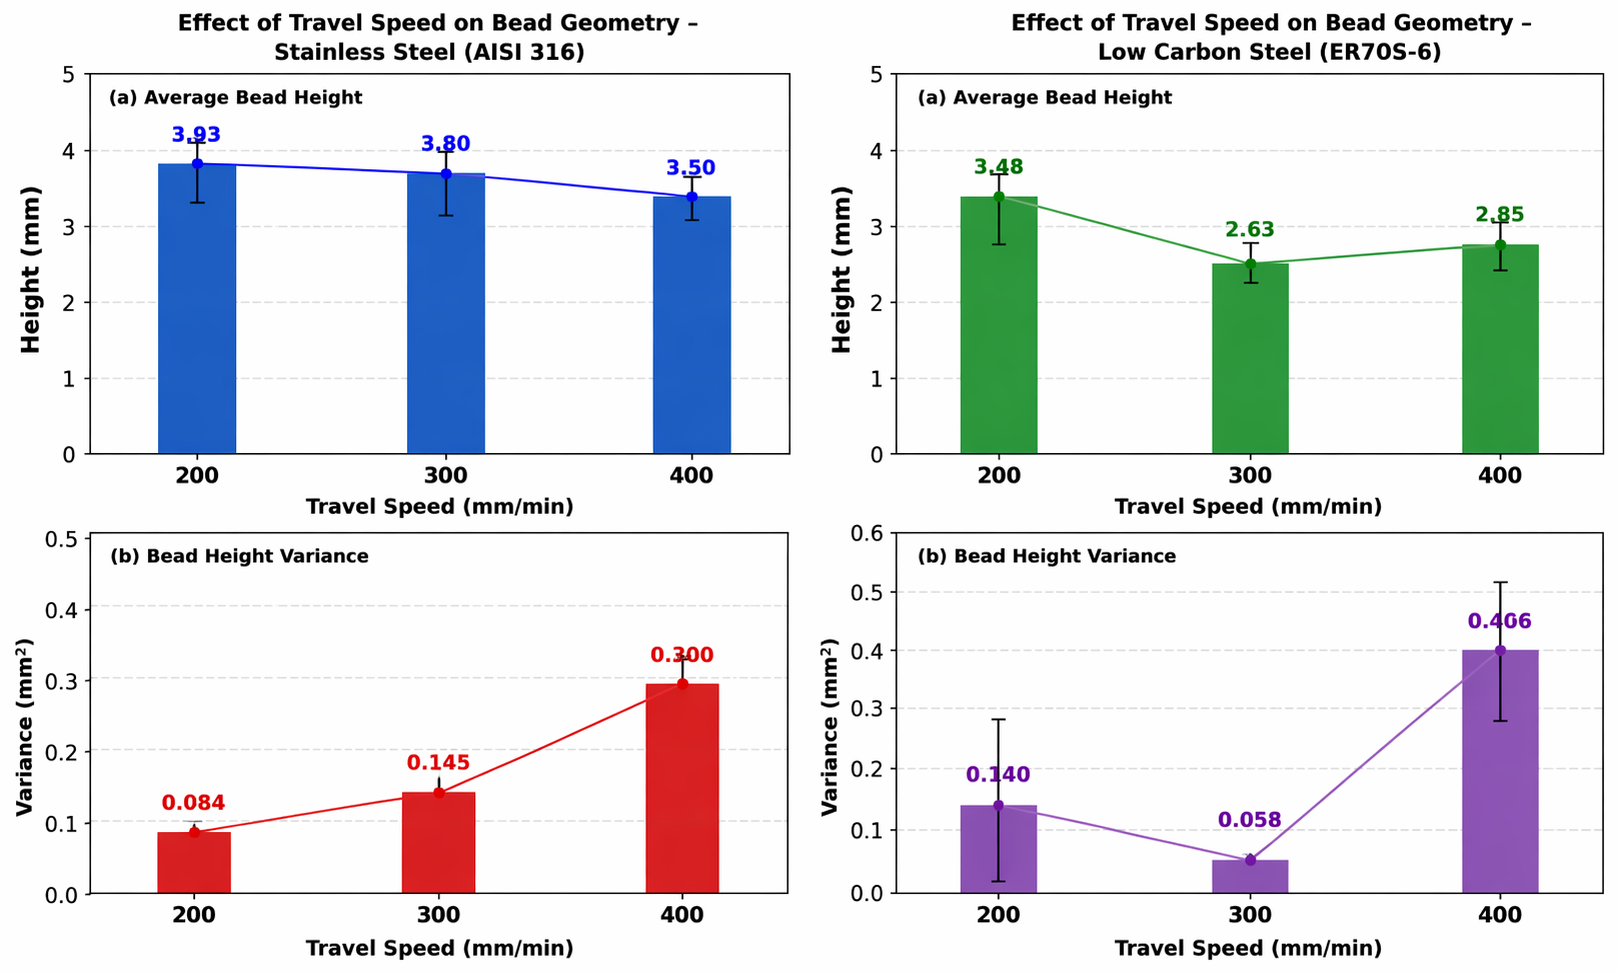
\includegraphics[width=1.95\textwidth,height=0.40\textheight,keepaspectratio]{CS8.png}
    \caption{Effect of travel speed (200, 300, and 400 mm/min) on bead geometry in stainless steel (left) and low carbon steel (right), showing variations in average bead height and height variance.}
    \label{fig:ts_effect_materials}
\end{figure*}


\begin{table*}[H]
\centering
\caption{Representative influence of travel speed on heat input and resulting bead geometry for stainless steel (AISI 316) and low carbon steel (ER70S-6) under fixed conditions ($V=12$ V, $I=150$ A, $\eta=0.8$).}
\label{tab:ts_geometry_comparison}
\begin{tabular}{c c c c c c c c}
\toprule
\textbf{TS} & \textbf{Heat Input} & \textbf{Material} & \textbf{Height} & \textbf{Width} & \textbf{$\sigma_h^2$} & \textbf{$\sigma_w^2$} & \textbf{Geometry Behavior} \\
\textbf{(mm/min)} & \textbf{(J/mm)} &  & \textbf{(mm)} & \textbf{(mm)} & \textbf{(mm$^2$)} & \textbf{(mm$^2$)} &  \\
\midrule
200 & 432 & AISI 316 & 2.8 & 7.4 & 0.35 & 0.50 & Large melt pool, strong spreading, reduced stability \\
200 & 432 & ER70S-6  & 3.4 & 6.2 & 0.20 & 0.25 & Moderate spreading, stable deposition \\
\midrule
300 & 288 & AISI 316 & 3.3 & 6.1 & 0.22 & 0.30 & Balanced geometry, improved consistency \\
300 & 288 & ER70S-6  & 3.7 & 5.5 & 0.15 & 0.20 & Controlled geometry, stable deposition \\
\midrule
400 & 216 & AISI 316 & 3.7 & 5.0 & 0.14 & 0.18 & Narrower bead, higher stability \\
400 & 216 & ER70S-6  & 4.0 & 4.8 & 0.10 & 0.14 & Confined bead, strong geometric stability \\
\bottomrule
\end{tabular}
\end{table*}


\begin{table*}[H]
\centering
\caption{Representative influence of travel speed on heat input and resulting bead geometry for stainless steel (AISI 316) and low carbon steel (ER70S-6) under fixed conditions ($V=12$ V, $I=150$ A, $\eta=0.8$).}
\label{tab:ts_geometry_comparison}
\begin{tabular}{c c c c c c c c}
\toprule
\textbf{TS} & \textbf{Heat Input} & \textbf{Material} & \textbf{Height} & \textbf{Width} & \textbf{$\sigma_h^2$} & \textbf{$\sigma_w^2$} & \textbf{Geometry Behavior} \\
\textbf{(mm/min)} & \textbf{(J/mm)} &  & \textbf{(mm)} & \textbf{(mm)} & \textbf{(mm$^2$)} & \textbf{(mm$^2$)} &  \\
\midrule
200 & 432 & AISI 316 & 2.8 & 7.4 & 0.35 & 0.50 & Large melt pool, strong spreading, reduced stability \\
200 & 432 & ER70S-6  & 3.4 & 6.2 & 0.20 & 0.25 & Moderate spreading, stable deposition \\
\midrule
300 & 288 & AISI 316 & 3.3 & 6.1 & 0.22 & 0.30 & Balanced geometry, improved consistency \\
300 & 288 & ER70S-6  & 3.7 & 5.5 & 0.15 & 0.20 & Controlled geometry, stable deposition \\
\midrule
400 & 216 & AISI 316 & 3.7 & 5.0 & 0.14 & 0.18 & Narrower bead, higher stability \\
400 & 216 & ER70S-6  & 4.0 & 4.8 & 0.10 & 0.14 & Confined bead, strong geometric stability \\
\bottomrule
\end{tabular}
\end{table*}



% =====================
\subsection{Effect of Contact Tip-to-Work Distance (CTWD)}

Contact tip-to-work distance (CTWD) influences the electrical resistance of the wire extension, which directly affects welding current and therefore heat input. As CTWD increases, electrical resistance increases, leading to a reduction in current. Consequently, the effective heat input decreases:

\begin{equation}
Q = \eta \frac{V I}{TS}
\end{equation}

For this analysis, the following experimental conditions are used:

\begin{equation}
V = 12 \text{ V}, \quad TS = 300 \text{ mm/min}, \quad \eta = 0.8
\end{equation}

The corresponding current values at different CTWD levels are:

\begin{equation}
\text{CTWD = 10 mm} \Rightarrow I \approx 170 \text{ A}
\end{equation}
\begin{equation}
\text{CTWD = 15 mm} \Rightarrow I \approx 150 \text{ A}
\end{equation}
\begin{equation}
\text{CTWD = 20 mm} \Rightarrow I \approx 130 \text{ A}
\end{equation}

Converting travel speed:

\begin{equation}
TS = 300 \text{ mm/min} = 5 \text{ mm/s}
\end{equation}

The resulting heat inputs are:

\begin{equation}
Q_{10} = 0.8 \times \frac{12 \times 170}{5} = 326 \text{ J/mm}
\end{equation}

\begin{equation}
Q_{15} = 0.8 \times \frac{12 \times 150}{5} = 288 \text{ J/mm}
\end{equation}

\begin{equation}
Q_{20} = 0.8 \times \frac{12 \times 130}{5} = 250 \text{ J/mm}
\end{equation}

\textbf{Stainless Steel (AISI 316):}

At \textbf{CTWD = 10 mm} ($Q \approx 326$ J/mm), the higher current produces a large melt pool with strong spreading. The bead height is approximately $3.0$ mm and width is approximately $7.0$ mm. Variances are elevated ($\sigma_h^2 \approx 0.30$, $\sigma_w^2 \approx 0.45$), indicating reduced stability.

At \textbf{CTWD = 15 mm} ($Q = 288$ J/mm), the melt pool becomes more controlled. The bead height increases slightly to $3.3$ mm, while width reduces to $6.1$ mm. Variances decrease ($\sigma_h^2 \approx 0.22$, $\sigma_w^2 \approx 0.30$).

At \textbf{CTWD = 20 mm} ($Q \approx 250$ J/mm), the reduced heat input produces a smaller melt pool. The bead height increases to approximately $3.6$ mm, while width reduces to approximately $5.3$ mm. Variances further decrease ($\sigma_h^2 \approx 0.15$, $\sigma_w^2 \approx 0.20$), indicating improved stability.

\textbf{Low Carbon Steel (ER70S-6):}

At \textbf{CTWD = 10 mm} ($Q \approx 326$ J/mm), the bead height is approximately $3.5$ mm and width is approximately $6.2$ mm. Variances remain moderate ($\sigma_h^2 \approx 0.18$, $\sigma_w^2 \approx 0.25$).

At \textbf{CTWD = 15 mm} ($Q = 288$ J/mm), the bead geometry stabilizes with height around $3.8$ mm and width around $5.5$ mm. Variances reduce slightly ($\sigma_h^2 \approx 0.14$, $\sigma_w^2 \approx 0.20$).

At \textbf{CTWD = 20 mm} ($Q \approx 250$ J/mm), the bead becomes more confined, with height approximately $4.1$ mm and width approximately $4.9$ mm. Variances remain low ($\sigma_h^2 \approx 0.10$, $\sigma_w^2 \approx 0.14$).

\paragraph{Interfacial Bonding and Detachability}

CTWD plays a critical role in determining the bonding strength of the first deposited layer. Lower CTWD values (e.g., 10 mm) produce higher heat input and deeper melt pool penetration into the substrate, resulting in strong metallurgical bonding and high adhesion.

In contrast, higher CTWD values (e.g., 20 mm) reduce heat input and limit substrate melting, resulting in weaker interfacial bonding. Under these conditions, the first deposited layer can be more easily detached from the substrate. This effect is more pronounced in stainless steel due to its heat retention, whereas low carbon steel maintains moderate bonding due to faster heat dissipation. So increasing CTWD reduces current and heat input, leading to smaller melt pools, reduced bead width, and increased bead height. In stainless steel, this significantly improves stability and reduces excessive spreading. In low carbon steel, the effect is more moderate due to efficient heat dissipation. Importantly, CTWD provides a practical control mechanism for interfacial behavior. The observed reduction in heat input with increasing CTWD suggests a potential pathway for reducing first-layer substrate bonding; direct interfacial mechanical testing is required to establish detachability. This makes CTWD, (as ahown in Fig.~\ref{fig:ctwd_effect_materials}), a critical parameter for applications requiring either permanent bonding or removable builds. Table~\ref{tab:ctwd_geometry}, summarizes the observation of CTWD in stainless steel and low carbon steel.

\begin{figure*}[!t]
    \centering
    \includegraphics[width=2.10\textwidth,height=0.50\textheight,keepaspectratio]{CTWD3.png}
    \caption{Effect of CTWD (10, 15, 20 mm) on bead geometry in stainless steel (left) and low carbon steel (right), showing variations in average bead height and height variance.}
    \label{fig:ctwd_effect_materials}
\end{figure*}

\begin{figure*}[!t]
    \centering
    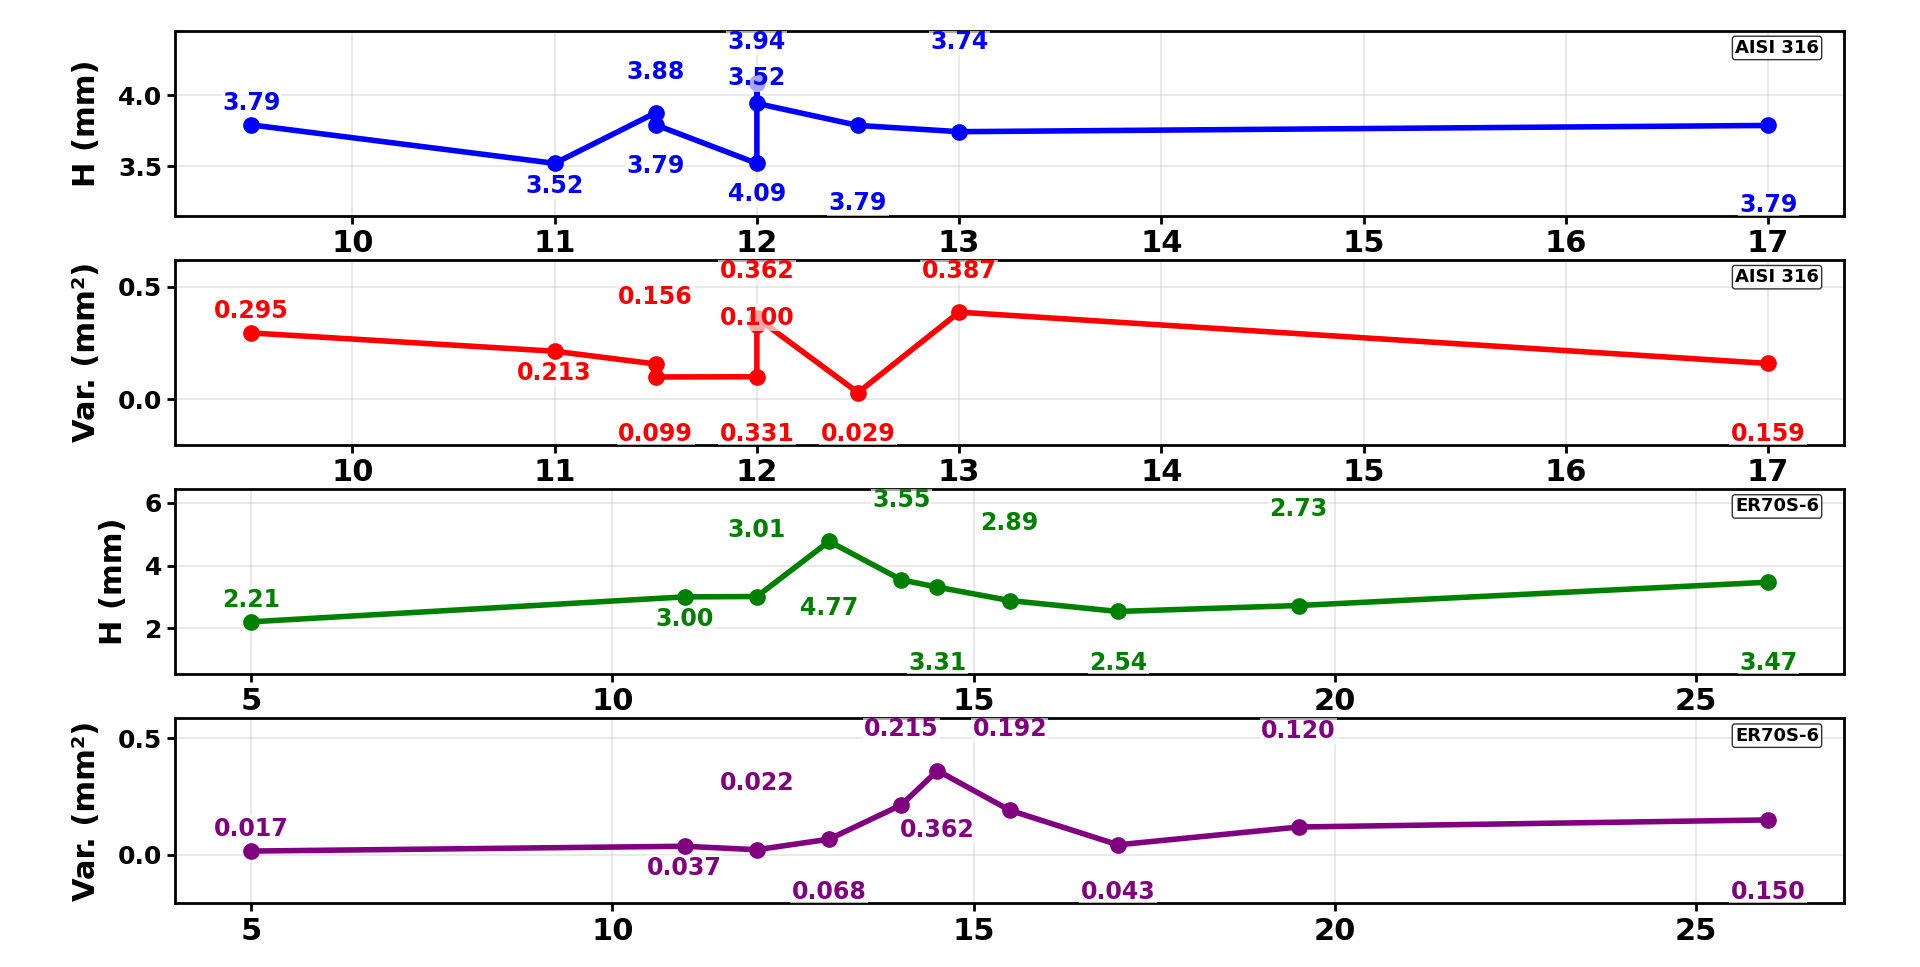
\includegraphics[width=1.95\textwidth,height=0.40\textheight,keepaspectratio]{CS4.png}
    \caption{Variation of CTWD on bead geometry in stainless steel (top) and low carbon steel (bottom), illustrating changes in average bead height and height variance across 10 mm, 15 mm, and 20 mm conditions.}
    \label{fig:ctwd_lowcarbon}
\end{figure*}

\begin{table*}[t]
\centering
\footnotesize
\setlength{\tabcolsep}{4pt}
\renewcommand{\arraystretch}{1.15}

\caption{Effect of contact tip-to-work distance (CTWD) on heat input and resulting geometry for stainless steel (AISI 316) and low carbon steel (ER70S-6) ($V=12$ V, $TS=300$ mm/min, $\eta=0.8$).}
\label{tab:ctwd_geometry}

\begin{tabular*}{\textwidth}{@{\extracolsep{\fill}} c c c c c c c c p{3.2cm}}
\toprule
\textbf{CTWD (mm)} & \textbf{Current (A)} & \textbf{Heat Input (J/mm)} & \textbf{Material} & \textbf{Height (mm)} & \textbf{Width (mm)} & $\boldsymbol{\sigma_h^2}$ & $\boldsymbol{\sigma_w^2}$ & \textbf{Geometry Behavior} \\
\midrule

10 & 170 & 326 & AISI 316 & 3.0 & 7.0 & 0.30 & 0.45 & Strong adhesion,deep penetration \\
10 & 170 & 326 & ER70S-6  & 3.5 & 6.2 & 0.18 & 0.25 & Strong bonding, moderate spreading \\

\midrule

15 & 150 & 288 & AISI 316 & 3.3 & 6.1 & 0.22 & 0.30 & Balanced bonding and geometry \\
15 & 150 & 288 & ER70S-6  & 3.8 & 5.5 & 0.14 & 0.20 & Stable interface, controlled spreading \\

\midrule

20 & 130 & 250 & AISI 316 & 3.6 & 5.3 & 0.15 & 0.20 & Reduced bonding, increased detachability \\
20 & 130 & 250 & ER70S-6  & 4.1 & 4.9 & 0.10 & 0.14 & Moderate detachability, stable geometry \\

\bottomrule
\end{tabular*}

\end{table*}


So increasing CTWD reduces current:
\begin{equation}
I \downarrow \Rightarrow Q \downarrow
\end{equation}

\textbf{Stainless Steel (AISI 316):}
\begin{itemize}
    \item Strong sensitivity in bead width
    \item Significant changes in melt pool size
\end{itemize}

\textbf{Low Carbon Steel (ER70S-6):}
\begin{itemize}
    \item Reduced sensitivity in width
    \item Primarily affects bead height and penetration
\end{itemize}

The reduced sensitivity in ER70S-6 is due to faster thermal dissipation limiting melt pool growth. Fig.~\ref{fig:ctwd_lowcarbon} shows the variation of CTWD on bead geometry.



\FloatBarrier


\begin{table*}[t]
\centering
\caption{Effect of voltage on heat input and resulting geometry for stainless steel (AISI 316) and low carbon steel (ER70S-6).}
\label{tab:voltage_effect}

\resizebox{\textwidth}{!}{%
\begin{tabular}{c c c c c c}
\toprule
\textbf{Voltage (V)} & \textbf{Rel. Heat Input $Q \propto \frac{V \cdot WFS}{TS}$} & \textbf{Material} & \textbf{Bead Height} & \textbf{Bead Width} & \textbf{Geometry Behavior} \\
\midrule

10 & Low & AISI 316 & High & Narrow & Limited spreading, stable but insufficient melting \\
10 & Low & ER70S-6  & Moderate-High & Narrower & Strong confinement due to rapid heat dissipation \\

\midrule

12 & Moderate & AISI 316 & Moderate & Moderate & Balanced geometry, controlled spreading \\
12 & Moderate & ER70S-6  & Moderate & Slightly Narrower & Stable deposition with reduced spreading \\

\midrule

16 & High & AISI 316 & Lower & Wide & Significant spreading, reduced stability, high melt pool fluidity \\
16 & High & ER70S-6  & Moderate & Moderate-Wide & Controlled spreading, improved stability \\

\bottomrule
\end{tabular}%
}

\end{table*}


\section{Geometry Analysis Summary}

In the previous sections, I presented the individual effects of voltage, wire feed speed, travel speed, and CTWD on bead height, width, and stability. 
To avoid repetition and to provide a clearer interpretation of how these parameters interact, I consolidate the results here using an integrated geometry–heat input perspective.

Table~\ref{tab:geom_summary} summarizes the combined trends across all experiments, linking each parameter to its influence on heat input, bead geometry, variance, and material response. 
This integrated view highlights how changes in process parameters propagate through the heat-input model and ultimately shape the geometric and stability outcomes for both ER70S-6 and AISI 316L.

\begin{table*}[t]
\centering
\caption{Integrated summary of parameter interactions with heat input, bead geometry, variance, and material-dependent response.}
\label{tab:geom_summary}

\resizebox{\textwidth}{!}{%
\begin{tabular}{c c c c c c}
\toprule
\textbf{Parameter} & \textbf{Heat Input} & \textbf{Bead Height} & \textbf{Bead Width} & \textbf{Variance} & \textbf{Material Response} \\
\midrule

Voltage & High with V & Lower at high V & Wider & Higher & 316L shows strong spreading; ER70S-6 remains more confined \\

\midrule

WFS & Increases current & Higher at low–mid WFS; lower at high WFS (316L) & Wider & Moderate increase & 316L becomes unstable at high WFS; ER70S-6 remains stable \\

\midrule

TS & Decreases with TS & Higher & Narrower & Higher at low TS & 316L highly heat-sensitive; ER70S-6 shows conservative changes \\

\midrule

CTWD & Decreases current & Higher & Narrower & Slight increase & 316L unstable at low CTWD; ER70S-6 maintains geometry \\

\bottomrule
\end{tabular}%
}

\end{table*}


This consolidated interpretation shows that geometry and stability cannot be understood from any single parameter in isolation. 
Instead, the combined effect of heat input and material thermal properties governs the observed trends. 
ER70S-6, with higher thermal conductivity, exhibits more conservative geometric changes and lower variance under parameter shifts, whereas AISI 316L shows stronger sensitivity and higher instability, especially under low travel speed and high voltage conditions.

By integrating the results into a single framework, Section~VII provides a clearer and less repetitive interpretation of how process parameters interact to shape bead geometry and deposition stability.







\section{Physics-Informed and Microstructural Interpretation}

The multivariable trends observed in this study can be further understood through fundamental heat transfer and melt pool physics. While process parameters such as voltage, wire feed speed (WFS), travel speed (TS), and contact tip-to-work distance (CTWD) directly influence heat input, the resulting geometric behavior is governed by material-dependent thermal transport and fluid flow mechanisms within the melt pool.

\subsection{Thermal Diffusion and Heat Retention}

The difference in geometric response between stainless steel (AISI 316) and low carbon steel (ER70S-6) can be interpreted in terms of thermal diffusion behavior. A useful dimensionless measure is the Fourier number:

\begin{equation}
Fo = \frac{\alpha t}{L^2}
\end{equation}

where $\alpha$ is the thermal diffusivity, $t$ is the characteristic thermal interaction time, and $L$ is a characteristic length scale of the melt pool.

Materials with higher thermal diffusivity, such as low-carbon steel (ER70S-6), exhibit faster heat dissipation and more efficient heat conduction compared to stainless steel, limiting melt pool growth and lateral spreading. This 
behavior is consistent with the faster heat dissipation observed in 
low-carbon steels, which promote more confined bead geometries 
compared to stainless steel \cite{fouad2025,debroy2018,Le2022}

In contrast, stainless steel (AISI 316) exhibits lower thermal diffusivity, resulting in lower effective Fourier numbers under similar processing conditions. This leads to localized heat accumulation, larger melt pools, and increased lateral spreading, which explains the wider beads and higher geometric variance observed experimentally.

\subsection{Melt Pool Flow and Surface-Driven Effects}

In addition to heat conduction, melt pool dynamics are significantly influenced by surface tension-driven flow, known as Marangoni convection. This phenomenon results from temperature gradients within the melt pool, where variations in surface tension cause fluid flow from lower to higher temperatures. The Marangoni effect plays a crucial role in melt pool stability, bead shape, and heat dissipation, and has been extensively studied in additive manufacturing processes like WAAM and LPBF \cite{fouad2025, chen2023waam_mech}

This behavior can be qualitatively described by the Marangoni effect, which governs the redistribution of molten material. Under higher heat input conditions, stronger temperature gradients enhance this flow, leading to increased lateral spreading of the melt  \cite{chen2023waam_mech,debroy2018}.

In stainless steel, where heat is retained for longer durations, sustained temperature gradients promote stronger Marangoni-driven flow, resulting in wider beads and increased variability. In contrast, the faster cooling rates in low carbon steel reduce the duration and intensity of these gradients, limiting melt pool flow and maintaining more confined bead geometries \cite{fouad2025,chen2023waam_mech,debroy2018,gao2026}.

\subsection{Cooling Rate and Microstructural Evolution}

The differences in heat input and thermal transport directly influence cooling rates, which play a critical role in determining the resulting microstructure of the deposited material. Higher heat input and slower cooling rates, as observed in stainless steel under low travel speed or high WFS conditions, tend to promote coarser grain structures due to extended solidification times. These conditions may also increase susceptibility to defects such as porosity or lack of uniform solidification due to melt pool instability.

Conversely, lower heat input and faster cooling rates, more characteristic of ER70S-6 under similar conditions, are expected to promote faster cooling and potentially finer microstructural features, although microstructural characterization was outside the scope of this study.


The more stable melt pool behavior observed in low carbon steel reduces fluctuations during solidification, contributing to lower geometric variance and potentially improved mechanical properties.
\begin{table}[t]
\centering
\caption{Experimental setup and operating conditions.}
\label{tab:experimental_setup}

\footnotesize
\setlength{\tabcolsep}{3pt}
\renewcommand{\arraystretch}{1.10}

\begin{tabular}{p{0.32\columnwidth} p{0.62\columnwidth}}
\toprule
\textbf{Parameter} & \textbf{Specification} \\
\midrule

Power source & Lincoln Electric Power Wave C300 \\
Process & GMAW-based WAAM \\
Wire diameter & 1.00 mm \\
Shielding gas & 98\% Ar / 2\% CO$_2$ \\
Gas flow rate & 15–20 L/min \\
Torch orientation & Perpendicular to travel direction \\
CTWD & 10–20 mm \\
Voltage range & 10–30 V \\
WFS range & 200–400 mm/min \\
Travel speed & 200–400 mm/min \\
Substrate dimensions & 100 $\times$ 100 $\times$ 6 mm \\
Total samples & 796 \\
Replicates & 3 per condition \\
Profilometer resolution & $\approx$1 $\mu$m vertical resolution \\
\bottomrule
\end{tabular}

\end{table}

\subsection{Implications for Process Stability and Material Performance}

The combined effects of thermal diffusion, melt pool convection, and cooling rate explain the strong material dependence observed in the process--geometry relationships \cite{chen2023waam_mech,fouad2025}. In stainless steel, heat retention and enhanced melt pool flow lead to increased spreading and higher geometric variability, which can negatively impact dimensional accuracy and structural consistency \cite{wang2023meltpool}. In low carbon steel, efficient heat dissipation promotes stable deposition, reduced variability, and improved control over bead geometry. Furthermore, the stability of the melt pool not only influences geometric consistency but also affects the integrity of the deposited material. Stable deposition conditions are associated with reduced defect formation and more uniform microstructures, while unstable conditions can introduce variability in both geometry and material properties.

\subsection{Material Thermophysical Properties}
\begin{table*}[t]
\centering
\caption{Thermophysical properties of materials used in this study.}
\label{tab:material_properties}

\resizebox{\textwidth}{!}{%
\begin{tabular}{l c c}
\toprule
\textbf{Property} & \textbf{AISI 316 Stainless Steel} & \textbf{ER70S-6 Low Carbon Steel} \\
\midrule
Thermal Conductivity, $k$ (W/m·K) & 14--16 & 45--60 \\
Specific Heat Capacity, $c_p$ (J/kg·K) & 480--500 & 470--490 \\
Density, $\rho$ (kg/m$^3$) & $\sim$8000 & $\sim$7850 \\
Thermal Diffusivity, $\alpha$ (mm$^2$/s) & $\sim$3--4 & $\sim$11--13 \\
Melting Temperature (°C) & 1375--1400 & 1450--1520 \\
Surface Tension Gradient (qualitative) & High sensitivity & Moderate sensitivity \\
\bottomrule
\end{tabular}%
}

\end{table*}
The geometric differences between AISI 316 and ER70S‑6 are strongly influenced by the thermophysical properties summarized in Table \ref{tab:material_properties}. The higher thermal conductivity and diffusivity of ER70S‑6 promote faster heat dissipation, producing more confined melt pools and improved stability. In contrast, the lower thermal diffusivity of AISI 316 leads to localized heat retention, larger melt pools, increased lateral spreading, and higher geometric variability.

Although thermal conductivity and diffusivity are major contributors, melt‑pool behavior in WAAM arises from multiple interacting factors—including electrical resistivity, arc characteristics, surface tension, viscosity, absorptivity, substrate condition, shielding gas composition, and deposition rate. These mechanisms are expected to influence the observed material‑dependent responses, although detailed thermal or microstructural characterization was outside the scope of this study.

Together, these effects explain the distinct geometric behavior of the two alloys under identical process conditions and support a material‑aware interpretation of parameter interactions in WAAM.

\section{Conclusion}

\begin{itemize}
    \item \textbf{Wire feed speed (WFS)} increases deposition rate and electrical current, thereby raising heat input and producing larger bead geometries.
    \item \textbf{Travel speed (TS)} reduces heat input per unit length, leading to narrower beads and less spreading, with instability emerging at very low TS.
    \item \textbf{Voltage} strongly influences melt-pool size and fluidity, with higher voltage producing wider beads and increased geometric variability.
    \item \textbf{CTWD} modifies current and heat input; larger CTWD reduces current and leads to smaller, more confined bead geometries.
    \item \textbf{Material properties} lead to substantially different geometric responses: AISI~316 shows greater spreading and instability due to lower thermal diffusivity, whereas ER70S-6 dissipates heat more rapidly and maintains more stable bead formation.
    \item \textbf{Variance-based metrics} provide an additional descriptor of deposition stability beyond mean geometry, revealing sensitivity to parameter interactions and material behavior.
\end{itemize}

\noindent\textbf{Overall Contribution:}  
This study provides a multivariable, physics-informed assessment of how voltage, WFS, TS, and CTWD collectively shape bead geometry and stability in WAAM. By integrating mean geometry with variance-based stability metrics and interpreting trends through material-dependent thermophysical behavior, the work establishes a material-aware foundation for more robust and predictive WAAM process optimization.

Importantly, the study shows that identical process inputs produce significantly different geometric outcomes across materials due to differences in thermophysical properties such as thermal conductivity and diffusivity. Stainless steel (AISI 316), with lower thermal conductivity, exhibits greater heat accumulation, larger melt pools, and higher geometric variability, whereas ER70S-6 demonstrates more confined bead profiles and improved stability due to efficient heat dissipation \cite{fouad2025,mulpur2026}. 

A key contribution of this work is the incorporation of variance-based metrics as indicators of deposition stability. Unlike traditional approaches that focus solely on mean geometric  \cite{Franke2025JIM,Kim2025WAAMVID}, the inclusion of variance enables identification of stable, marginal, and unstable deposition regimes, providing a more robust framework for process evaluation and parameter selection. 

Furthermore, the results show that CTWD functions as an effective lever for controlling first‑layer adhesion. Lower CTWD increases current and heat input, promoting stronger metallurgical bonding, whereas higher CTWD reduces heat input and enables controlled detachability when needed. This provides a practical means of tailoring substrate adhesion in WAAM. More broadly, the findings establish a material‑aware process–geometry framework that supports informed parameter selection and stable bead formation, enabling future advances in predictive modeling, inverse design, and closed‑loop control for data‑driven WAAM operation.

\section*{Acknowledgment}
The authors gratefully acknowledge the support and resources provided by Case Western Reserve University. This work was supported in part by NASA under the University Student Research Challenge (USRC), the National Science Foundation through the HAMMER Engineering Research Center (ERC) under award number EEC-2133630, and Lincoln Electric. The authors also acknowledge the Advanced Manufacturing and Mechanical Reliability Center (AMMRC) and the Institute for Smart, Secure, and Connected Systems (ISSACS) for providing the facilities, infrastructure, and technical support essential to this experimental study.  The authors further thank collaborators and research colleagues who contributed to the development, operation, and maintenance of the WAAM experimental platform and metrology systems. Their support was instrumental in enabling the large-scale experimental data acquisition and analysis presented in this work.

\section*{Data and Code Availability}

The experimental datasets, bead-geometry measurements, and variance metrics used in this study are publicly available at:
\texttt{[insert DOI or URL]}.

All code used for data processing, statistical analysis, and figure generation is openly accessible at:
\texttt{[insert GitHub/Zenodo link]}.

These materials enable full reproducibility of the results and support further research on multivariable WAAM process modeling.

\section*{Author Contributions}

B.~Ebika designed the experimental study, performed the WAAM trials, collected the bead-geometry data, and led the analysis. 
V.~Ramasamy contributed to the experimental design, data interpretation, and physics-informed process analysis. 
J.~Lewandowski provided guidance on material behavior and metallurgical interpretation. 
K.~Loparo supervised the project, while contributing to the statistical framework, variance-based stability analysis, and multivariable modeling strategy. 
J.~Ekeamadi contributed to conceptual development, and supported manuscript preparation. 

All authors reviewed, edited, and approved the final manuscript.


\section*{Conflict of Interest}

The authors declare that they have no known competing financial interests or personal relationships that could have influenced the work reported in this study. This research was conducted as part of academic and federally supported programs, and no commercial or financial conflicts are associated with this work.




% =========================
% REFERENCES
% =========================
\bibliographystyle{elsarticle-num}
\bibliography{references}


% Option B: Manual references (uncomment if you don't want BibTeX)
% \begin{thebibliography}{00}
% \bibitem{ding2015} D. Ding \emph{et al.}, ``Wire-feed additive manufacturing: A review,'' \emph{Int. J. Adv. Manuf. Technol.}, 2015.
% \bibitem{montgomery} D. C. Montgomery, \emph{Design and Analysis of Experiments}. Wiley, 2017.
% \end{thebibliography}


\end{document}